\documentclass[twoside]{book}

% Packages required by doxygen
\usepackage{fixltx2e}
\usepackage{calc}
\usepackage{doxygen}
\usepackage[export]{adjustbox} % also loads graphicx
\usepackage{graphicx}
\usepackage[utf8]{inputenc}
\usepackage{makeidx}
\usepackage{multicol}
\usepackage{multirow}
\PassOptionsToPackage{warn}{textcomp}
\usepackage{textcomp}
\usepackage[nointegrals]{wasysym}
\usepackage[table]{xcolor}

% Font selection
\usepackage[T1]{fontenc}
\usepackage[scaled=.90]{helvet}
\usepackage{courier}
\usepackage{amssymb}
\usepackage{sectsty}
\renewcommand{\familydefault}{\sfdefault}
\allsectionsfont{%
  \fontseries{bc}\selectfont%
  \color{darkgray}%
}
\renewcommand{\DoxyLabelFont}{%
  \fontseries{bc}\selectfont%
  \color{darkgray}%
}
\newcommand{\+}{\discretionary{\mbox{\scriptsize$\hookleftarrow$}}{}{}}

% Page & text layout
\usepackage{geometry}
\geometry{%
  a4paper,%
  top=2.5cm,%
  bottom=2.5cm,%
  left=2.5cm,%
  right=2.5cm%
}
\tolerance=750
\hfuzz=15pt
\hbadness=750
\setlength{\emergencystretch}{15pt}
\setlength{\parindent}{0cm}
\setlength{\parskip}{3ex plus 2ex minus 2ex}
\makeatletter
\renewcommand{\paragraph}{%
  \@startsection{paragraph}{4}{0ex}{-1.0ex}{1.0ex}{%
    \normalfont\normalsize\bfseries\SS@parafont%
  }%
}
\renewcommand{\subparagraph}{%
  \@startsection{subparagraph}{5}{0ex}{-1.0ex}{1.0ex}{%
    \normalfont\normalsize\bfseries\SS@subparafont%
  }%
}
\makeatother

% Headers & footers
\usepackage{fancyhdr}
\pagestyle{fancyplain}
\fancyhead[LE]{\fancyplain{}{\bfseries\thepage}}
\fancyhead[CE]{\fancyplain{}{}}
\fancyhead[RE]{\fancyplain{}{\bfseries\leftmark}}
\fancyhead[LO]{\fancyplain{}{\bfseries\rightmark}}
\fancyhead[CO]{\fancyplain{}{}}
\fancyhead[RO]{\fancyplain{}{\bfseries\thepage}}
\fancyfoot[LE]{\fancyplain{}{}}
\fancyfoot[CE]{\fancyplain{}{}}
\fancyfoot[RE]{\fancyplain{}{\bfseries\scriptsize Generated by Doxygen }}
\fancyfoot[LO]{\fancyplain{}{\bfseries\scriptsize Generated by Doxygen }}
\fancyfoot[CO]{\fancyplain{}{}}
\fancyfoot[RO]{\fancyplain{}{}}
\renewcommand{\footrulewidth}{0.4pt}
\renewcommand{\chaptermark}[1]{%
  \markboth{#1}{}%
}
\renewcommand{\sectionmark}[1]{%
  \markright{\thesection\ #1}%
}

% Indices & bibliography
\usepackage{natbib}
\usepackage[titles]{tocloft}
\setcounter{tocdepth}{3}
\setcounter{secnumdepth}{5}
\makeindex

% Hyperlinks (required, but should be loaded last)
\usepackage{ifpdf}
\ifpdf
  \usepackage[pdftex,pagebackref=true]{hyperref}
\else
  \usepackage[ps2pdf,pagebackref=true]{hyperref}
\fi
\hypersetup{%
  colorlinks=true,%
  linkcolor=blue,%
  citecolor=blue,%
  unicode%
}

% Custom commands
\newcommand{\clearemptydoublepage}{%
  \newpage{\pagestyle{empty}\cleardoublepage}%
}

\usepackage{caption}
\captionsetup{labelsep=space,justification=centering,font={bf},singlelinecheck=off,skip=4pt,position=top}

%===== C O N T E N T S =====

\begin{document}

% Titlepage & ToC
\hypersetup{pageanchor=false,
             bookmarksnumbered=true,
             pdfencoding=unicode
            }
\pagenumbering{alph}
\begin{titlepage}
\vspace*{7cm}
\begin{center}%
{\Large Charge Tracker }\\
\vspace*{1cm}
{\large Generated by Doxygen 1.8.14}\\
\end{center}
\end{titlepage}
\clearemptydoublepage
\pagenumbering{roman}
\tableofcontents
\clearemptydoublepage
\pagenumbering{arabic}
\hypersetup{pageanchor=true}

%--- Begin generated contents ---
\chapter{Charge Tracker Documentation}
\label{index}\hypertarget{index}{}This is the documentation for the \href{https://github.com/ritstudentgovernment/chargeflask}{\tt Charge\+Tracker} backend, the front-\/end documentation is located in the \href{https://github.com/ritstudentgovernment/chargevue}{\tt chargevue} repository.\hypertarget{index_gettingstarted}{}\section{Getting Started}\label{index_gettingstarted}
This guide contains step-\/by-\/step instructions on how to install the server, how to get data to the backend and how to get data from it.\hypertarget{index_serverinstall}{}\subsection{Server Installation}\label{index_serverinstall}
Prerequisites\+: Flask and Postgre\+S\+QL
\begin{DoxyEnumerate}
\item Pull project from \href{https://github.com/ritstudentgovernment/chargeflask}{\tt this repo}.
\item Install and create \href{http://python-guide-pt-br.readthedocs.io/en/latest/dev/virtualenvs/}{\tt virtual environment}.
\item Create a database for the project.
\item Specify the {\ttfamily S\+Q\+L\+A\+L\+C\+H\+E\+M\+Y\+\_\+\+D\+A\+T\+A\+B\+A\+S\+E\+\_\+\+U\+RI} in the {\ttfamily config.\+py} file with the database path.
\item Activate virtual environment.
\item Execute {\ttfamily pip install -\/r requirements.\+txt}
\item Complete the {\ttfamily secrets.\+py} file (Contact System Administrator for relevant data).
\item Run {\ttfamily python run.\+py}
\end{DoxyEnumerate}\hypertarget{index_testutil}{}\subsection{Testing Utilities}\label{index_testutil}
In some cases, you\textquotesingle{}d like to test if your backend code is properly working. But, because you don\textquotesingle{}t have access to a frontend yet, it might seem quite hard to test your code while developing it. For this, it\textquotesingle{}s recommended to install in your machine a tool called \href{https://electronjs.org/apps/socket-io-tester}{\tt Socket.\+io tester}, which let\textquotesingle{}s so send and retrieve data from the backend without the need of a developed client.\hypertarget{index_datamani}{}\section{Data Manipulation}\label{index_datamani}
Charge\+Tracker uses a technology called \href{https://socket.io/}{\tt Socket\+IO}, which basically provides real-\/time communication between two different machines through Web\+Sockets. Socket\+IO allows the easy implementation of Web\+Sockets cross-\/platform and cross-\/language. For example, the \href{https://github.com/ritstudentgovernment/chargevue}{\tt chargevue} client for this application, uses the native Javascript Socket\+IO library, meanwhile this backend utilizes the Flask library \href{https://flask-socketio.readthedocs.io/en/latest/}{\tt Flask-\/\+Socket\+IO}. Bellow, there are a few detailed examples on how to request or submit data to and from the Charge\+Tracker backend.\hypertarget{index_submitData}{}\subsection{Submitting Data}\label{index_submitData}
Submitting data to Charge\+Tracker is very simple. Basically, inside each the controllers file of each module there are certain functions that {\itshape listen} for data in a specific event name. For example, inside the controllers of the Committees module, we can see the {\ttfamily get\+\_\+commitees} method\+:


\begin{DoxyCode}
##
##  Gets list of all committees.
##
##@param broadcast  Flag to broadcast list of committees to all users.
##
## @emit       Emits a list of committees.
##
@socketio.on('get\_committees')
def get\_committees(broadcast = False):
    committees = Committees.query.filter\_by(enabled = True).all()
    comm\_ser = [\{"id": c.id, "title": c.title\} for c in committees]
    emit("get\_committees", comm\_ser, broadcast= broadcast)
\end{DoxyCode}


We can see that every method inside the controllers start with the line `.on('$<$event\+\_\+name$>$\textquotesingle{}){\ttfamily , this basically means that once the server listens to a request in that specific event, the function under it will be executed. In this case, when a person sends a request with the event}get\+\_\+committees\`{} to the server, the function get\+\_\+committees will be executed.

To send this request to the server, the request can be written in the following way\+:


\begin{DoxyCode}
// Javascript Socket-IO request.
var socket = io.connect('http://localhost:5000');
socket.emit('get\_committees');
\end{DoxyCode}


We can also notice that the {\ttfamily get\+\_\+committees} method gets the parameter broadcast, which basically broadcasts the list of committees to all the users listening, to send data to the server, you can send a J\+S\+ON object or a String.

For example, if I want my request of committees to be broadcasted to everyone that is listening to {\ttfamily get\+\_\+committees}, I can do\+:


\begin{DoxyCode}
// Javascript Socket-IO request with params.
var socket = io.connect('http://localhost:5000');
socket.emit('get\_committees', true);
\end{DoxyCode}
\hypertarget{index_retrieveData}{}\subsection{Retrieving Data}\label{index_retrieveData}
{\bfseries I\+M\+P\+O\+R\+T\+A\+NT}\+: Also take into account that to receive this data, you have to be listening to the events with the same event\+\_\+name. So, if I\textquotesingle{}d like to receive all the committees, you have to listen to the {\ttfamily get\+\_\+committees} event name\+:


\begin{DoxyCode}
// Javascript Socket-IO listener.
var socket = io.connect('http://localhost:5000');
socket.on('get\_committees', function(data)\{
    console.log(data);
\});
\end{DoxyCode}


These channels are always open, so you only have to listen to data once and you\textquotesingle{}ll keep receiving new data as it becomes available, without having to create new requests!\hypertarget{index_modulestruct}{}\section{Module Structure}\label{index_modulestruct}
To keep the source code organized, each functionality of \href{https://github.com/ritstudentgovernment/chargeflask}{\tt Charge\+Tracker} is divided in different modules. For example, the Users module contains everything relevant to user authentication, meanwhile the Committees module has everything relevant to manipulating committees.

Every module in Charge\+Tracker contains the following files\+:


\begin{DoxyItemize}
\item {\ttfamily \+\_\+\+\_\+init\+\_\+\+\_\+.\+py} (required)\+: This file is usually empty, its necessary to create a Python module.
\item {\ttfamily models.\+py} (required)\+: This file contains the model declaration of the module itself. This usually contains the S\+Q\+L\+Alchemy model declaration.
\item {\ttfamily controllers.\+py} (required)\+: This file contains all the relevant controllers to manipulate data on the server, please refer to the examples on the \href{#datamani}{\tt Data Manipulation} section.
\item {\ttfamily test\+\_\+$<$module\+\_\+name$>$.py} (required)\+: This file contains all the test cases for this specific module, please refer to the examples on the Testing Modules section.
\item {\ttfamily $<$module\+\_\+name$>$\+\_\+response.\+py}\+: Instead of hard-\/coding response strings inside the controllers class, all the response strings specific to this module are located inside this class. In the future, this will allow the easy implementation of \href{https://github.com/ritstudentgovernment/chargeflask}{\tt Charge\+Tracker} in a different language.
\end{DoxyItemize}\hypertarget{index_unittests}{}\section{Unit Tests and Code Coverage}\label{index_unittests}
Every module in this project is unit tested to check if the code implemented is fully functional. For unit testing, Charge\+Tracker utilizes the Python testing utility, \href{https://docs.pytest.org}{\tt pytest}. To execute your unit tests locally, you can simply run the command\+: {\ttfamily py.\+test -\/-\/cov=./app}, if you want to generate a html coverage report, the same command can be executed with the flag {\ttfamily -\/-\/cov-\/report=html}. For code coverage, this project uses \href{https://travis-ci.org/}{\tt Travis\+CI} and \href{https://codecov.io/gh}{\tt Codecov}, the Travis\+CI .yml file is located under {\ttfamily .travis.\+yml}, which basically contains the configuration that Travis needs to execute your code. Also, take into account that Travis\+CI needs a copy of your {\ttfamily secrets.\+py} to execute your code, this is done by encrypting your secrets file with Travis\+CI. 
\chapter{Namespace Index}
\section{Namespace List}
Here is a list of all documented namespaces with brief descriptions\+:\begin{DoxyCompactList}
\item\contentsline{section}{\mbox{\hyperlink{namespaceapp}{app}} }{\pageref{namespaceapp}}{}
\item\contentsline{section}{\mbox{\hyperlink{namespaceapp_1_1actions_1_1models}{app.\+actions.\+models}} }{\pageref{namespaceapp_1_1actions_1_1models}}{}
\item\contentsline{section}{\mbox{\hyperlink{namespaceapp_1_1charges_1_1controllers}{app.\+charges.\+controllers}} }{\pageref{namespaceapp_1_1charges_1_1controllers}}{}
\item\contentsline{section}{\mbox{\hyperlink{namespaceapp_1_1charges_1_1models}{app.\+charges.\+models}} }{\pageref{namespaceapp_1_1charges_1_1models}}{}
\item\contentsline{section}{\mbox{\hyperlink{namespaceapp_1_1committees_1_1controllers}{app.\+committees.\+controllers}} }{\pageref{namespaceapp_1_1committees_1_1controllers}}{}
\item\contentsline{section}{\mbox{\hyperlink{namespaceapp_1_1committees_1_1models}{app.\+committees.\+models}} }{\pageref{namespaceapp_1_1committees_1_1models}}{}
\item\contentsline{section}{\mbox{\hyperlink{namespaceapp_1_1invitations_1_1controllers}{app.\+invitations.\+controllers}} }{\pageref{namespaceapp_1_1invitations_1_1controllers}}{}
\item\contentsline{section}{\mbox{\hyperlink{namespaceapp_1_1invitations_1_1models}{app.\+invitations.\+models}} }{\pageref{namespaceapp_1_1invitations_1_1models}}{}
\item\contentsline{section}{\mbox{\hyperlink{namespaceapp_1_1members_1_1controllers}{app.\+members.\+controllers}} }{\pageref{namespaceapp_1_1members_1_1controllers}}{}
\item\contentsline{section}{\mbox{\hyperlink{namespaceapp_1_1members_1_1models}{app.\+members.\+models}} }{\pageref{namespaceapp_1_1members_1_1models}}{}
\item\contentsline{section}{\mbox{\hyperlink{namespaceapp_1_1notes_1_1models}{app.\+notes.\+models}} }{\pageref{namespaceapp_1_1notes_1_1models}}{}
\item\contentsline{section}{\mbox{\hyperlink{namespaceapp_1_1users_1_1controllers}{app.\+users.\+controllers}} }{\pageref{namespaceapp_1_1users_1_1controllers}}{}
\item\contentsline{section}{\mbox{\hyperlink{namespaceapp_1_1users_1_1models}{app.\+users.\+models}} }{\pageref{namespaceapp_1_1users_1_1models}}{}
\item\contentsline{section}{\mbox{\hyperlink{namespaceapp_1_1users_1_1permissions}{app.\+users.\+permissions}} }{\pageref{namespaceapp_1_1users_1_1permissions}}{}
\end{DoxyCompactList}

\chapter{Hierarchical Index}
\section{Class Hierarchy}
This inheritance list is sorted roughly, but not completely, alphabetically\+:\begin{DoxyCompactList}
\item Model\begin{DoxyCompactList}
\item \contentsline{section}{app.\+actions.\+models.\+Actions}{\pageref{classapp_1_1actions_1_1models_1_1_actions}}{}
\item \contentsline{section}{app.\+charges.\+models.\+Charges}{\pageref{classapp_1_1charges_1_1models_1_1_charges}}{}
\item \contentsline{section}{app.\+committees.\+models.\+Committees}{\pageref{classapp_1_1committees_1_1models_1_1_committees}}{}
\item \contentsline{section}{app.\+invitations.\+models.\+Invitations}{\pageref{classapp_1_1invitations_1_1models_1_1_invitations}}{}
\item \contentsline{section}{app.\+notes.\+models.\+Notes}{\pageref{classapp_1_1notes_1_1models_1_1_notes}}{}
\item \contentsline{section}{app.\+users.\+models.\+Users}{\pageref{classapp_1_1users_1_1models_1_1_users}}{}
\end{DoxyCompactList}
\item \contentsline{section}{app.\+users.\+permissions.\+Permissions}{\pageref{classapp_1_1users_1_1permissions_1_1_permissions}}{}
\item Enum\begin{DoxyCompactList}
\item \contentsline{section}{app.\+charges.\+models.\+Priority\+Type}{\pageref{classapp_1_1charges_1_1models_1_1_priority_type}}{}
\item \contentsline{section}{app.\+charges.\+models.\+Status\+Type}{\pageref{classapp_1_1charges_1_1models_1_1_status_type}}{}
\end{DoxyCompactList}
\end{DoxyCompactList}

\chapter{Class Index}
\section{Class List}
Here are the classes, structs, unions and interfaces with brief descriptions\+:\begin{DoxyCompactList}
\item\contentsline{section}{\mbox{\hyperlink{classapp_1_1actions_1_1models_1_1_actions}{app.\+actions.\+models.\+Actions}} }{\pageref{classapp_1_1actions_1_1models_1_1_actions}}{}
\item\contentsline{section}{\mbox{\hyperlink{classapp_1_1charges_1_1models_1_1_charges}{app.\+charges.\+models.\+Charges}} \\*\mbox{\hyperlink{classapp_1_1charges_1_1models_1_1_charges}{Charges}} Model }{\pageref{classapp_1_1charges_1_1models_1_1_charges}}{}
\item\contentsline{section}{\mbox{\hyperlink{classapp_1_1committees_1_1models_1_1_committees}{app.\+committees.\+models.\+Committees}} }{\pageref{classapp_1_1committees_1_1models_1_1_committees}}{}
\item\contentsline{section}{\mbox{\hyperlink{classapp_1_1invitations_1_1models_1_1_invitations}{app.\+invitations.\+models.\+Invitations}} }{\pageref{classapp_1_1invitations_1_1models_1_1_invitations}}{}
\item\contentsline{section}{\mbox{\hyperlink{classapp_1_1notes_1_1models_1_1_notes}{app.\+notes.\+models.\+Notes}} }{\pageref{classapp_1_1notes_1_1models_1_1_notes}}{}
\item\contentsline{section}{\mbox{\hyperlink{classapp_1_1users_1_1permissions_1_1_permissions}{app.\+users.\+permissions.\+Permissions}} \\*Permission categories for users }{\pageref{classapp_1_1users_1_1permissions_1_1_permissions}}{}
\item\contentsline{section}{\mbox{\hyperlink{classapp_1_1charges_1_1models_1_1_priority_type}{app.\+charges.\+models.\+Priority\+Type}} \\*Levels of priority for charges }{\pageref{classapp_1_1charges_1_1models_1_1_priority_type}}{}
\item\contentsline{section}{\mbox{\hyperlink{classapp_1_1charges_1_1models_1_1_status_type}{app.\+charges.\+models.\+Status\+Type}} \\*Status types for charges }{\pageref{classapp_1_1charges_1_1models_1_1_status_type}}{}
\item\contentsline{section}{\mbox{\hyperlink{classapp_1_1users_1_1models_1_1_users}{app.\+users.\+models.\+Users}} }{\pageref{classapp_1_1users_1_1models_1_1_users}}{}
\end{DoxyCompactList}

\chapter{Namespace Documentation}
\hypertarget{namespaceapp}{}\section{app Namespace Reference}
\label{namespaceapp}\index{app@{app}}
\subsection*{Variables}
\begin{DoxyCompactItemize}
\item 
\mbox{\Hypertarget{namespaceapp_a675b4ea702c13dc4b8c05f985a25b496}\label{namespaceapp_a675b4ea702c13dc4b8c05f985a25b496}} 
{\bfseries app} = Flask(\+\_\+\+\_\+name\+\_\+\+\_\+, template\+\_\+folder=\textquotesingle{}static\textquotesingle{})
\item 
\mbox{\Hypertarget{namespaceapp_a5e96f78557153399b3460b769e9bfeac}\label{namespaceapp_a5e96f78557153399b3460b769e9bfeac}} 
{\bfseries socketio} = Socket\+IO(app)
\item 
\mbox{\Hypertarget{namespaceapp_a75341a4bc0e8e239f299316136af3466}\label{namespaceapp_a75341a4bc0e8e239f299316136af3466}} 
{\bfseries db} = S\+Q\+L\+Alchemy(app)
\item 
\mbox{\Hypertarget{namespaceapp_a476241c29a05353b264621894d7c23bb}\label{namespaceapp_a476241c29a05353b264621894d7c23bb}} 
{\bfseries mail} = Mail(app)
\end{DoxyCompactItemize}


\subsection{Detailed Description}
\begin{DoxyVerb}filename: __init__.py
description: Initiate Charge Tracker app
created by: Omar De La Hoz (oed7416@rit.edu)
created on: 09/07/17
\end{DoxyVerb}
 
\hypertarget{namespaceapp_1_1actions_1_1models}{}\section{app.\+actions.\+models Namespace Reference}
\label{namespaceapp_1_1actions_1_1models}\index{app.\+actions.\+models@{app.\+actions.\+models}}
\subsection*{Classes}
\begin{DoxyCompactItemize}
\item 
class \mbox{\hyperlink{classapp_1_1actions_1_1models_1_1_actions}{Actions}}
\end{DoxyCompactItemize}


\subsection{Detailed Description}
\begin{DoxyVerb}filename: models.py
description: Model for Charge Actions.
created by: Omar De La Hoz (oed7416@rit.edu)
created on: 09/05/17
\end{DoxyVerb}
 
\hypertarget{namespaceapp_1_1charges_1_1controllers}{}\section{app.\+charges.\+controllers Namespace Reference}
\label{namespaceapp_1_1charges_1_1controllers}\index{app.\+charges.\+controllers@{app.\+charges.\+controllers}}
\subsection*{Functions}
\begin{DoxyCompactItemize}
\item 
def \mbox{\hyperlink{namespaceapp_1_1charges_1_1controllers_a30141a884cf96a10060458e66e74aca9}{get\+\_\+charges}} (committee\+\_\+id, broadcast=False)
\begin{DoxyCompactList}\small\item\em Gets the charges for a specific committee. \end{DoxyCompactList}\item 
def \mbox{\hyperlink{namespaceapp_1_1charges_1_1controllers_acde694db95925313933db3ab5ebc3ad0}{get\+\_\+charge}} (charge\+\_\+id, broadcast=False)
\begin{DoxyCompactList}\small\item\em Gets a charge by its ID. \end{DoxyCompactList}\item 
def \mbox{\hyperlink{namespaceapp_1_1charges_1_1controllers_a5376e63b039cd45d5faae35d1d50d55b}{create\+\_\+charge}} (user\+\_\+data)
\begin{DoxyCompactList}\small\item\em Creates a charge for a Committee. \end{DoxyCompactList}\end{DoxyCompactItemize}


\subsection{Detailed Description}
\begin{DoxyVerb}filename: controllers.py
description: Cronrollers for charges.
created by: Omar De La Hoz (oed7416@rit.edu)
created on: 12/05/17
\end{DoxyVerb}
 

\subsection{Function Documentation}
\mbox{\Hypertarget{namespaceapp_1_1charges_1_1controllers_a5376e63b039cd45d5faae35d1d50d55b}\label{namespaceapp_1_1charges_1_1controllers_a5376e63b039cd45d5faae35d1d50d55b}} 
\index{app\+::charges\+::controllers@{app\+::charges\+::controllers}!create\+\_\+charge@{create\+\_\+charge}}
\index{create\+\_\+charge@{create\+\_\+charge}!app\+::charges\+::controllers@{app\+::charges\+::controllers}}
\subsubsection{\texorpdfstring{create\+\_\+charge()}{create\_charge()}}
{\footnotesize\ttfamily def app.\+charges.\+controllers.\+create\+\_\+charge (\begin{DoxyParamCaption}\item[{}]{user\+\_\+data }\end{DoxyParamCaption})}



Creates a charge for a Committee. 

A charge for a committee is created, the default status for the charge will be Unapproved, which means that the charge is a Charge Initiative.


\begin{DoxyParams}{Parameters}
{\em user\+\_\+data} & The user data to create a charge for a committee. This can include\+:\\
\hline
\end{DoxyParams}

\begin{DoxyItemize}
\item token (required)\+: Token of creator.
\item title (required)\+: Charge title.
\item committee (required)\+: The charge\textquotesingle{}s committee.
\item priority (required)\+: The charge\textquotesingle{}s priority.
\item description\+: The purpose of the charge.
\item objectives\+: The objectives of a charge (Array).
\end{DoxyItemize}

\begin{DoxyReturn}{Returns}
\{ description\+\_\+of\+\_\+the\+\_\+return\+\_\+value \} 
\end{DoxyReturn}
\mbox{\Hypertarget{namespaceapp_1_1charges_1_1controllers_acde694db95925313933db3ab5ebc3ad0}\label{namespaceapp_1_1charges_1_1controllers_acde694db95925313933db3ab5ebc3ad0}} 
\index{app\+::charges\+::controllers@{app\+::charges\+::controllers}!get\+\_\+charge@{get\+\_\+charge}}
\index{get\+\_\+charge@{get\+\_\+charge}!app\+::charges\+::controllers@{app\+::charges\+::controllers}}
\subsubsection{\texorpdfstring{get\+\_\+charge()}{get\_charge()}}
{\footnotesize\ttfamily def app.\+charges.\+controllers.\+get\+\_\+charge (\begin{DoxyParamCaption}\item[{}]{charge\+\_\+id,  }\item[{}]{broadcast = {\ttfamily False} }\end{DoxyParamCaption})}



Gets a charge by its ID. 


\begin{DoxyParams}{Parameters}
{\em charge\+\_\+id} & The charge identifier \\
\hline
{\em broadcast} & Flag to broadcast list of charges to all users.\\
\hline
\end{DoxyParams}
An objet containing the detailed view of a charge. \mbox{\Hypertarget{namespaceapp_1_1charges_1_1controllers_a30141a884cf96a10060458e66e74aca9}\label{namespaceapp_1_1charges_1_1controllers_a30141a884cf96a10060458e66e74aca9}} 
\index{app\+::charges\+::controllers@{app\+::charges\+::controllers}!get\+\_\+charges@{get\+\_\+charges}}
\index{get\+\_\+charges@{get\+\_\+charges}!app\+::charges\+::controllers@{app\+::charges\+::controllers}}
\subsubsection{\texorpdfstring{get\+\_\+charges()}{get\_charges()}}
{\footnotesize\ttfamily def app.\+charges.\+controllers.\+get\+\_\+charges (\begin{DoxyParamCaption}\item[{}]{committee\+\_\+id,  }\item[{}]{broadcast = {\ttfamily False} }\end{DoxyParamCaption})}



Gets the charges for a specific committee. 


\begin{DoxyParams}{Parameters}
{\em committee\+\_\+id} & The committee identifier \\
\hline
{\em broadcast} & Flag to broadcast list of charges to all users.\\
\hline
\end{DoxyParams}
Emits a list of charges for committee. 
\hypertarget{namespaceapp_1_1charges_1_1models}{}\section{app.\+charges.\+models Namespace Reference}
\label{namespaceapp_1_1charges_1_1models}\index{app.\+charges.\+models@{app.\+charges.\+models}}
\subsection*{Classes}
\begin{DoxyCompactItemize}
\item 
class \mbox{\hyperlink{classapp_1_1charges_1_1models_1_1_charges}{Charges}}
\begin{DoxyCompactList}\small\item\em \mbox{\hyperlink{classapp_1_1charges_1_1models_1_1_charges}{Charges}} Model. \end{DoxyCompactList}\item 
class \mbox{\hyperlink{classapp_1_1charges_1_1models_1_1_priority_type}{Priority\+Type}}
\begin{DoxyCompactList}\small\item\em Levels of priority for charges. \end{DoxyCompactList}\item 
class \mbox{\hyperlink{classapp_1_1charges_1_1models_1_1_status_type}{Status\+Type}}
\begin{DoxyCompactList}\small\item\em Status types for charges. \end{DoxyCompactList}\end{DoxyCompactItemize}


\subsection{Detailed Description}
\begin{DoxyVerb}filename: charges.py
description: Model for charges.
created by: Omar De La Hoz (oed7416@rit.edu)
created on: 08/30/17
\end{DoxyVerb}
 
\hypertarget{namespaceapp_1_1committees_1_1controllers}{}\section{app.\+committees.\+controllers Namespace Reference}
\label{namespaceapp_1_1committees_1_1controllers}\index{app.\+committees.\+controllers@{app.\+committees.\+controllers}}
\subsection*{Functions}
\begin{DoxyCompactItemize}
\item 
def \mbox{\hyperlink{namespaceapp_1_1committees_1_1controllers_a13062ac4ed1e797b5015282df19f6171}{get\+\_\+committees}} (broadcast=False)
\begin{DoxyCompactList}\small\item\em Gets list of all committees. \end{DoxyCompactList}\item 
def \mbox{\hyperlink{namespaceapp_1_1committees_1_1controllers_a3583100187139ebf105b562438e9bf7a}{get\+\_\+permissions}} (user\+\_\+data)
\begin{DoxyCompactList}\small\item\em Get a users permissions for a specific committee. \end{DoxyCompactList}\item 
def \mbox{\hyperlink{namespaceapp_1_1committees_1_1controllers_a85c678c4dc91cc884de63f2a7d8b3b52}{get\+\_\+committee}} (committee\+\_\+id, broadcast=False)
\begin{DoxyCompactList}\small\item\em Gets a specific committee by its id. \end{DoxyCompactList}\item 
def \mbox{\hyperlink{namespaceapp_1_1committees_1_1controllers_a43d988c96e26843d6b0fa328bfbfca5e}{create\+\_\+committee}} (user\+\_\+data)
\begin{DoxyCompactList}\small\item\em Creates a committee. \end{DoxyCompactList}\item 
def \mbox{\hyperlink{namespaceapp_1_1committees_1_1controllers_a1be50a5e100f6e73441b49cda5fef1e0}{edit\+\_\+committee}} (user\+\_\+data)
\begin{DoxyCompactList}\small\item\em Edits a committee (Must be admin user) \end{DoxyCompactList}\end{DoxyCompactItemize}


\subsection{Detailed Description}
\begin{DoxyVerb}filename: controllers.py
description: Controller for Committees.
created by: Omar De La Hoz (oed7416@rit.edu)
created on: 09/19/17
\end{DoxyVerb}
 

\subsection{Function Documentation}
\mbox{\Hypertarget{namespaceapp_1_1committees_1_1controllers_a43d988c96e26843d6b0fa328bfbfca5e}\label{namespaceapp_1_1committees_1_1controllers_a43d988c96e26843d6b0fa328bfbfca5e}} 
\index{app\+::committees\+::controllers@{app\+::committees\+::controllers}!create\+\_\+committee@{create\+\_\+committee}}
\index{create\+\_\+committee@{create\+\_\+committee}!app\+::committees\+::controllers@{app\+::committees\+::controllers}}
\subsubsection{\texorpdfstring{create\+\_\+committee()}{create\_committee()}}
{\footnotesize\ttfamily def app.\+committees.\+controllers.\+create\+\_\+committee (\begin{DoxyParamCaption}\item[{}]{user\+\_\+data }\end{DoxyParamCaption})}



Creates a committee. 

(Must be admin user)


\begin{DoxyParams}{Parameters}
{\em user\+\_\+data} & The user data required to create a committee. \begin{DoxyVerb}                    All the following fields are required:

                    token - Token of the current user
                    title - The title of the new committee 
                    head - Head of committee (Must exist in app)
                    description - Description of new committee
                    location - Location of committee meetings
                    meeting_time - Time of committee meeting
                    meeting_day - Day of the week of committee meeting
\end{DoxyVerb}
\\
\hline
\end{DoxyParams}
Emits a success message if created, error if not. \mbox{\Hypertarget{namespaceapp_1_1committees_1_1controllers_a1be50a5e100f6e73441b49cda5fef1e0}\label{namespaceapp_1_1committees_1_1controllers_a1be50a5e100f6e73441b49cda5fef1e0}} 
\index{app\+::committees\+::controllers@{app\+::committees\+::controllers}!edit\+\_\+committee@{edit\+\_\+committee}}
\index{edit\+\_\+committee@{edit\+\_\+committee}!app\+::committees\+::controllers@{app\+::committees\+::controllers}}
\subsubsection{\texorpdfstring{edit\+\_\+committee()}{edit\_committee()}}
{\footnotesize\ttfamily def app.\+committees.\+controllers.\+edit\+\_\+committee (\begin{DoxyParamCaption}\item[{}]{user\+\_\+data }\end{DoxyParamCaption})}



Edits a committee (Must be admin user) 


\begin{DoxyParams}{Parameters}
{\em user\+\_\+data} & The user data to edit a committee, must contain a token and any of the following fields\+:
\begin{DoxyItemize}
\item description
\item head
\item location
\item meeting\+\_\+time
\item enabled
\item committee\+\_\+img
\end{DoxyItemize}\\
\hline
\end{DoxyParams}
Any other field will be ignored.

Emits a success mesage if edited, errors otherwise. \mbox{\Hypertarget{namespaceapp_1_1committees_1_1controllers_a85c678c4dc91cc884de63f2a7d8b3b52}\label{namespaceapp_1_1committees_1_1controllers_a85c678c4dc91cc884de63f2a7d8b3b52}} 
\index{app\+::committees\+::controllers@{app\+::committees\+::controllers}!get\+\_\+committee@{get\+\_\+committee}}
\index{get\+\_\+committee@{get\+\_\+committee}!app\+::committees\+::controllers@{app\+::committees\+::controllers}}
\subsubsection{\texorpdfstring{get\+\_\+committee()}{get\_committee()}}
{\footnotesize\ttfamily def app.\+committees.\+controllers.\+get\+\_\+committee (\begin{DoxyParamCaption}\item[{}]{committee\+\_\+id,  }\item[{}]{broadcast = {\ttfamily False} }\end{DoxyParamCaption})}



Gets a specific committee by its id. 


\begin{DoxyParams}{Parameters}
{\em committee\+\_\+id} & The committee identifier\\
\hline
\end{DoxyParams}
An object containing a detailed view of a specific committee. \mbox{\Hypertarget{namespaceapp_1_1committees_1_1controllers_a13062ac4ed1e797b5015282df19f6171}\label{namespaceapp_1_1committees_1_1controllers_a13062ac4ed1e797b5015282df19f6171}} 
\index{app\+::committees\+::controllers@{app\+::committees\+::controllers}!get\+\_\+committees@{get\+\_\+committees}}
\index{get\+\_\+committees@{get\+\_\+committees}!app\+::committees\+::controllers@{app\+::committees\+::controllers}}
\subsubsection{\texorpdfstring{get\+\_\+committees()}{get\_committees()}}
{\footnotesize\ttfamily def app.\+committees.\+controllers.\+get\+\_\+committees (\begin{DoxyParamCaption}\item[{}]{broadcast = {\ttfamily False} }\end{DoxyParamCaption})}



Gets list of all committees. 


\begin{DoxyParams}{Parameters}
{\em broadcast} & Flag to broadcast list of committees to all users.\\
\hline
\end{DoxyParams}
Emits a list of committees. \mbox{\Hypertarget{namespaceapp_1_1committees_1_1controllers_a3583100187139ebf105b562438e9bf7a}\label{namespaceapp_1_1committees_1_1controllers_a3583100187139ebf105b562438e9bf7a}} 
\index{app\+::committees\+::controllers@{app\+::committees\+::controllers}!get\+\_\+permissions@{get\+\_\+permissions}}
\index{get\+\_\+permissions@{get\+\_\+permissions}!app\+::committees\+::controllers@{app\+::committees\+::controllers}}
\subsubsection{\texorpdfstring{get\+\_\+permissions()}{get\_permissions()}}
{\footnotesize\ttfamily def app.\+committees.\+controllers.\+get\+\_\+permissions (\begin{DoxyParamCaption}\item[{}]{user\+\_\+data }\end{DoxyParamCaption})}



Get a users permissions for a specific committee. 


\begin{DoxyParams}{Parameters}
{\em user\+\_\+data} & Contains user \char`\"{}token\char`\"{} (optional) and \char`\"{}id\char`\"{} of committee. (required.)\\
\hline
\end{DoxyParams}
Integer describing the user permissions. 
\hypertarget{namespaceapp_1_1committees_1_1models}{}\section{app.\+committees.\+models Namespace Reference}
\label{namespaceapp_1_1committees_1_1models}\index{app.\+committees.\+models@{app.\+committees.\+models}}
\subsection*{Classes}
\begin{DoxyCompactItemize}
\item 
class \mbox{\hyperlink{classapp_1_1committees_1_1models_1_1_committees}{Committees}}
\end{DoxyCompactItemize}


\subsection{Detailed Description}
\begin{DoxyVerb}filename: committees.py
description: Model for Committees.
created by: Omar De La Hoz (oed7416@rit.edu)
created on: 08/31/17
\end{DoxyVerb}
 
\hypertarget{namespaceapp_1_1invitations_1_1controllers}{}\section{app.\+invitations.\+controllers Namespace Reference}
\label{namespaceapp_1_1invitations_1_1controllers}\index{app.\+invitations.\+controllers@{app.\+invitations.\+controllers}}
\subsection*{Functions}
\begin{DoxyCompactItemize}
\item 
def \mbox{\hyperlink{namespaceapp_1_1invitations_1_1controllers_ac9d6b41452741ffa83fd04f7f935dd4b}{send\+\_\+invite}} (new\+\_\+user, committee)
\begin{DoxyCompactList}\small\item\em Sends an invitation to join a committee when user doesn\textquotesingle{}t exist in Charge\+Tracker. \end{DoxyCompactList}\item 
def \mbox{\hyperlink{namespaceapp_1_1invitations_1_1controllers_a41239d3a243861515a5a14599333ad0e}{send\+\_\+request}} (new\+\_\+user, committee)
\begin{DoxyCompactList}\small\item\em Sends a request email to join a committee to the committee head. \end{DoxyCompactList}\item 
def \mbox{\hyperlink{namespaceapp_1_1invitations_1_1controllers_aec05f77e1fcf926dfc05239d1272e3e3}{get\+\_\+invitation}} (user\+\_\+data)
\begin{DoxyCompactList}\small\item\em Gets the data for a specific invitation/request. \end{DoxyCompactList}\item 
def \mbox{\hyperlink{namespaceapp_1_1invitations_1_1controllers_a5bc2456a1f82dd8c9c0942dfdfbda935}{set\+\_\+invitation}} (user\+\_\+data)
\begin{DoxyCompactList}\small\item\em Changes the status of an invitation/request. \end{DoxyCompactList}\end{DoxyCompactItemize}


\subsection{Detailed Description}
\begin{DoxyVerb}filename: controllers.py
description: Controllers for email invitations.
created by: Omar De La Hoz (oed7416@rit.edu)
created on: 10/12/17
\end{DoxyVerb}
 

\subsection{Function Documentation}
\mbox{\Hypertarget{namespaceapp_1_1invitations_1_1controllers_aec05f77e1fcf926dfc05239d1272e3e3}\label{namespaceapp_1_1invitations_1_1controllers_aec05f77e1fcf926dfc05239d1272e3e3}} 
\index{app\+::invitations\+::controllers@{app\+::invitations\+::controllers}!get\+\_\+invitation@{get\+\_\+invitation}}
\index{get\+\_\+invitation@{get\+\_\+invitation}!app\+::invitations\+::controllers@{app\+::invitations\+::controllers}}
\subsubsection{\texorpdfstring{get\+\_\+invitation()}{get\_invitation()}}
{\footnotesize\ttfamily def app.\+invitations.\+controllers.\+get\+\_\+invitation (\begin{DoxyParamCaption}\item[{}]{user\+\_\+data }\end{DoxyParamCaption})}



Gets the data for a specific invitation/request. 


\begin{DoxyParams}{Parameters}
{\em user\+\_\+data} & The data to display a specific invitation, contains the keys (all required)\+:
\begin{DoxyItemize}
\item token\+: The token of the authenticated user
\item invitation\+\_\+id\+: Id of invitation/request.
\end{DoxyItemize}\\
\hline
\end{DoxyParams}
Data of a specific invitation or errors. \mbox{\Hypertarget{namespaceapp_1_1invitations_1_1controllers_ac9d6b41452741ffa83fd04f7f935dd4b}\label{namespaceapp_1_1invitations_1_1controllers_ac9d6b41452741ffa83fd04f7f935dd4b}} 
\index{app\+::invitations\+::controllers@{app\+::invitations\+::controllers}!send\+\_\+invite@{send\+\_\+invite}}
\index{send\+\_\+invite@{send\+\_\+invite}!app\+::invitations\+::controllers@{app\+::invitations\+::controllers}}
\subsubsection{\texorpdfstring{send\+\_\+invite()}{send\_invite()}}
{\footnotesize\ttfamily def app.\+invitations.\+controllers.\+send\+\_\+invite (\begin{DoxyParamCaption}\item[{}]{new\+\_\+user,  }\item[{}]{committee }\end{DoxyParamCaption})}



Sends an invitation to join a committee when user doesn\textquotesingle{}t exist in Charge\+Tracker. 


\begin{DoxyParams}{Parameters}
{\em committee} & The committee to join. \\
\hline
{\em new\+\_\+user} & The user to be invited.\\
\hline
\end{DoxyParams}
\begin{DoxyReturn}{Returns}
True if email sent, False if not. 
\end{DoxyReturn}
\mbox{\Hypertarget{namespaceapp_1_1invitations_1_1controllers_a41239d3a243861515a5a14599333ad0e}\label{namespaceapp_1_1invitations_1_1controllers_a41239d3a243861515a5a14599333ad0e}} 
\index{app\+::invitations\+::controllers@{app\+::invitations\+::controllers}!send\+\_\+request@{send\+\_\+request}}
\index{send\+\_\+request@{send\+\_\+request}!app\+::invitations\+::controllers@{app\+::invitations\+::controllers}}
\subsubsection{\texorpdfstring{send\+\_\+request()}{send\_request()}}
{\footnotesize\ttfamily def app.\+invitations.\+controllers.\+send\+\_\+request (\begin{DoxyParamCaption}\item[{}]{new\+\_\+user,  }\item[{}]{committee }\end{DoxyParamCaption})}



Sends a request email to join a committee to the committee head. 


\begin{DoxyParams}{Parameters}
{\em new\+\_\+user} & The user to be added. \\
\hline
{\em committee} & The committee to join.\\
\hline
\end{DoxyParams}
\begin{DoxyReturn}{Returns}
True if email sent, False if not. 
\end{DoxyReturn}
\mbox{\Hypertarget{namespaceapp_1_1invitations_1_1controllers_a5bc2456a1f82dd8c9c0942dfdfbda935}\label{namespaceapp_1_1invitations_1_1controllers_a5bc2456a1f82dd8c9c0942dfdfbda935}} 
\index{app\+::invitations\+::controllers@{app\+::invitations\+::controllers}!set\+\_\+invitation@{set\+\_\+invitation}}
\index{set\+\_\+invitation@{set\+\_\+invitation}!app\+::invitations\+::controllers@{app\+::invitations\+::controllers}}
\subsubsection{\texorpdfstring{set\+\_\+invitation()}{set\_invitation()}}
{\footnotesize\ttfamily def app.\+invitations.\+controllers.\+set\+\_\+invitation (\begin{DoxyParamCaption}\item[{}]{user\+\_\+data }\end{DoxyParamCaption})}



Changes the status of an invitation/request. 


\begin{DoxyParams}{Parameters}
{\em user\+\_\+data} & The data to modify a specific invitation, contains the keys (all required)\+:
\begin{DoxyItemize}
\item token\+: The token of the authenticated user
\item invitation\+\_\+id\+: Id of invitation/request.
\item status\+: True to accept, false otherwise.
\end{DoxyItemize}\\
\hline
\end{DoxyParams}
User\+Added, Invite\+Deleted or errors. 
\hypertarget{namespaceapp_1_1invitations_1_1models}{}\section{app.\+invitations.\+models Namespace Reference}
\label{namespaceapp_1_1invitations_1_1models}\index{app.\+invitations.\+models@{app.\+invitations.\+models}}
\subsection*{Classes}
\begin{DoxyCompactItemize}
\item 
class \mbox{\hyperlink{classapp_1_1invitations_1_1models_1_1_invitations}{Invitations}}
\end{DoxyCompactItemize}


\subsection{Detailed Description}
\begin{DoxyVerb}filename: models.py
description: Model for committee invitations.
created by: Omar De La Hoz (oed7416@rit.edu)
created on: 10/19/17
\end{DoxyVerb}
 
\hypertarget{namespaceapp_1_1members_1_1controllers}{}\section{app.\+members.\+controllers Namespace Reference}
\label{namespaceapp_1_1members_1_1controllers}\index{app.\+members.\+controllers@{app.\+members.\+controllers}}
\subsection*{Functions}
\begin{DoxyCompactItemize}
\item 
def \mbox{\hyperlink{namespaceapp_1_1members_1_1controllers_aa5952443267e1c04b380a533a4e4ea7f}{get\+\_\+committee\+\_\+members}} (committee\+\_\+id, broadcast=False)
\begin{DoxyCompactList}\small\item\em Gets the committee members for a specific committee. \end{DoxyCompactList}\item 
def \mbox{\hyperlink{namespaceapp_1_1members_1_1controllers_a8999f221f1849949968973c73a4ff409}{add\+\_\+to\+\_\+committee}} (user\+\_\+data)
\begin{DoxyCompactList}\small\item\em Adds to committee. \end{DoxyCompactList}\item 
def \mbox{\hyperlink{namespaceapp_1_1members_1_1controllers_a76a53b46e9b3997b5fac18a82280fce2}{remove\+\_\+from\+\_\+committee}} (user\+\_\+data)
\begin{DoxyCompactList}\small\item\em Removes a member from a committee. \end{DoxyCompactList}\end{DoxyCompactItemize}


\subsection{Detailed Description}
\begin{DoxyVerb}filename: controllers.py
description: Controllers for Memberships.
created by: Omar De La Hoz (oed7416@rit.edu)
created on: 09/26/17
\end{DoxyVerb}
 

\subsection{Function Documentation}
\mbox{\Hypertarget{namespaceapp_1_1members_1_1controllers_a8999f221f1849949968973c73a4ff409}\label{namespaceapp_1_1members_1_1controllers_a8999f221f1849949968973c73a4ff409}} 
\index{app\+::members\+::controllers@{app\+::members\+::controllers}!add\+\_\+to\+\_\+committee@{add\+\_\+to\+\_\+committee}}
\index{add\+\_\+to\+\_\+committee@{add\+\_\+to\+\_\+committee}!app\+::members\+::controllers@{app\+::members\+::controllers}}
\subsubsection{\texorpdfstring{add\+\_\+to\+\_\+committee()}{add\_to\_committee()}}
{\footnotesize\ttfamily def app.\+members.\+controllers.\+add\+\_\+to\+\_\+committee (\begin{DoxyParamCaption}\item[{}]{user\+\_\+data }\end{DoxyParamCaption})}



Adds to committee. 


\begin{DoxyParams}{Parameters}
{\em user\+\_\+data} & Contains the data needed to add a member to a committee. This can contain\+:\\
\hline
\end{DoxyParams}

\begin{DoxyItemize}
\item token (required)\+: Token of current user.
\item user\+\_\+id (optional)\+: Id of user to be added, if not specified, current user will be added to committee.
\item committee\+\_\+id (required)\+: Id of committee.
\end{DoxyItemize}

Any other parameters will be ignored.

Success if user could be added to committee, error if not. \mbox{\Hypertarget{namespaceapp_1_1members_1_1controllers_aa5952443267e1c04b380a533a4e4ea7f}\label{namespaceapp_1_1members_1_1controllers_aa5952443267e1c04b380a533a4e4ea7f}} 
\index{app\+::members\+::controllers@{app\+::members\+::controllers}!get\+\_\+committee\+\_\+members@{get\+\_\+committee\+\_\+members}}
\index{get\+\_\+committee\+\_\+members@{get\+\_\+committee\+\_\+members}!app\+::members\+::controllers@{app\+::members\+::controllers}}
\subsubsection{\texorpdfstring{get\+\_\+committee\+\_\+members()}{get\_committee\_members()}}
{\footnotesize\ttfamily def app.\+members.\+controllers.\+get\+\_\+committee\+\_\+members (\begin{DoxyParamCaption}\item[{}]{committee\+\_\+id,  }\item[{}]{broadcast = {\ttfamily False} }\end{DoxyParamCaption})}



Gets the committee members for a specific committee. 


\begin{DoxyParams}{Parameters}
{\em committee\+\_\+id} & The id for the committee.\\
\hline
\end{DoxyParams}
Array with committee members. \mbox{\Hypertarget{namespaceapp_1_1members_1_1controllers_a76a53b46e9b3997b5fac18a82280fce2}\label{namespaceapp_1_1members_1_1controllers_a76a53b46e9b3997b5fac18a82280fce2}} 
\index{app\+::members\+::controllers@{app\+::members\+::controllers}!remove\+\_\+from\+\_\+committee@{remove\+\_\+from\+\_\+committee}}
\index{remove\+\_\+from\+\_\+committee@{remove\+\_\+from\+\_\+committee}!app\+::members\+::controllers@{app\+::members\+::controllers}}
\subsubsection{\texorpdfstring{remove\+\_\+from\+\_\+committee()}{remove\_from\_committee()}}
{\footnotesize\ttfamily def app.\+members.\+controllers.\+remove\+\_\+from\+\_\+committee (\begin{DoxyParamCaption}\item[{}]{user\+\_\+data }\end{DoxyParamCaption})}



Removes a member from a committee. 


\begin{DoxyParams}{Parameters}
{\em user\+\_\+data} & Contains the data needed to add a member to a committee. This can contain\+:\\
\hline
\end{DoxyParams}

\begin{DoxyItemize}
\item token (required)\+: Token of current user.
\item user\+\_\+id (required)\+: Id of user to be deleted.
\item committee\+\_\+id (required)\+: Id of committee.
\end{DoxyItemize}

Any other parameters will be ignored.

Success if member could be deleted, error if not. 
\hypertarget{namespaceapp_1_1members_1_1models}{}\section{app.\+members.\+models Namespace Reference}
\label{namespaceapp_1_1members_1_1models}\index{app.\+members.\+models@{app.\+members.\+models}}
\subsection*{Variables}
\begin{DoxyCompactItemize}
\item 
{\bfseries members\+\_\+table}
\end{DoxyCompactItemize}


\subsection{Detailed Description}
\begin{DoxyVerb}filename: members.py
description: Model for Members in Committees.
created by: Omar De La Hoz (oed7416@rit.edu)
created on: 08/31/17
\end{DoxyVerb}
 

\subsection{Variable Documentation}
\mbox{\Hypertarget{namespaceapp_1_1members_1_1models_a0a54bcbc283b250025eed1d910e0071d}\label{namespaceapp_1_1members_1_1models_a0a54bcbc283b250025eed1d910e0071d}} 
\index{app\+::members\+::models@{app\+::members\+::models}!members\+\_\+table@{members\+\_\+table}}
\index{members\+\_\+table@{members\+\_\+table}!app\+::members\+::models@{app\+::members\+::models}}
\subsubsection{\texorpdfstring{members\+\_\+table}{members\_table}}
{\footnotesize\ttfamily app.\+members.\+models.\+members\+\_\+table}

{\bfseries Initial value\+:}
\begin{DoxyCode}
1 =  db.Table(\textcolor{stringliteral}{'members'}, db.Model.metadata,
2     db.Column(\textcolor{stringliteral}{'committees\_id'}, db.String(255), db.ForeignKey(\textcolor{stringliteral}{'committees.id'})),
3     db.Column(\textcolor{stringliteral}{'users\_id'}, db.String(255), db.ForeignKey(\textcolor{stringliteral}{'users.id'}))
4 )
\end{DoxyCode}

\hypertarget{namespaceapp_1_1notes_1_1models}{}\section{app.\+notes.\+models Namespace Reference}
\label{namespaceapp_1_1notes_1_1models}\index{app.\+notes.\+models@{app.\+notes.\+models}}
\subsection*{Classes}
\begin{DoxyCompactItemize}
\item 
class \mbox{\hyperlink{classapp_1_1notes_1_1models_1_1_notes}{Notes}}
\end{DoxyCompactItemize}


\subsection{Detailed Description}
\begin{DoxyVerb}filename: models.py
description: Models for Charge Notes.
created by: Omar De La Hoz (oed7416@rit.edu)
created on: 09/05/17
\end{DoxyVerb}
 
\hypertarget{namespaceapp_1_1users_1_1controllers}{}\section{app.\+users.\+controllers Namespace Reference}
\label{namespaceapp_1_1users_1_1controllers}\index{app.\+users.\+controllers@{app.\+users.\+controllers}}
\subsection*{Functions}
\begin{DoxyCompactItemize}
\item 
\mbox{\Hypertarget{namespaceapp_1_1users_1_1controllers_a65452c24918bbf57d6208a8146d9b685}\label{namespaceapp_1_1users_1_1controllers_a65452c24918bbf57d6208a8146d9b685}} 
def {\bfseries login\+\_\+user} (credentials)
\end{DoxyCompactItemize}


\subsection{Detailed Description}
\begin{DoxyVerb}filename: controllers.py
description: Controller for Users.
created by: Omar De La Hoz (oed7416@rit.edu)
created on: 09/07/17
\end{DoxyVerb}
 
\hypertarget{namespaceapp_1_1users_1_1models}{}\section{app.\+users.\+models Namespace Reference}
\label{namespaceapp_1_1users_1_1models}\index{app.\+users.\+models@{app.\+users.\+models}}
\subsection*{Classes}
\begin{DoxyCompactItemize}
\item 
class \mbox{\hyperlink{classapp_1_1users_1_1models_1_1_users}{Users}}
\end{DoxyCompactItemize}


\subsection{Detailed Description}
\begin{DoxyVerb}filename: models.py
description: Model for Users.
created by: Omar De La Hoz (oed7416@rit.edu)
created on: 08/31/17
\end{DoxyVerb}
 
\hypertarget{namespaceapp_1_1users_1_1permissions}{}\section{app.\+users.\+permissions Namespace Reference}
\label{namespaceapp_1_1users_1_1permissions}\index{app.\+users.\+permissions@{app.\+users.\+permissions}}
\subsection*{Classes}
\begin{DoxyCompactItemize}
\item 
class \mbox{\hyperlink{classapp_1_1users_1_1permissions_1_1_permissions}{Permissions}}
\begin{DoxyCompactList}\small\item\em Permission categories for users. \end{DoxyCompactList}\end{DoxyCompactItemize}


\subsection{Detailed Description}
\begin{DoxyVerb}filename: permissions.py
description: User permissions for
created by: Omar De La Hoz (oed7416@rit.edu)
created on: 10/26/17
\end{DoxyVerb}
 
\chapter{Class Documentation}
\hypertarget{classapp_1_1actions_1_1models_1_1_actions}{}\section{app.\+actions.\+models.\+Actions Class Reference}
\label{classapp_1_1actions_1_1models_1_1_actions}\index{app.\+actions.\+models.\+Actions@{app.\+actions.\+models.\+Actions}}
Inheritance diagram for app.\+actions.\+models.\+Actions\+:\begin{figure}[H]
\begin{center}
\leavevmode
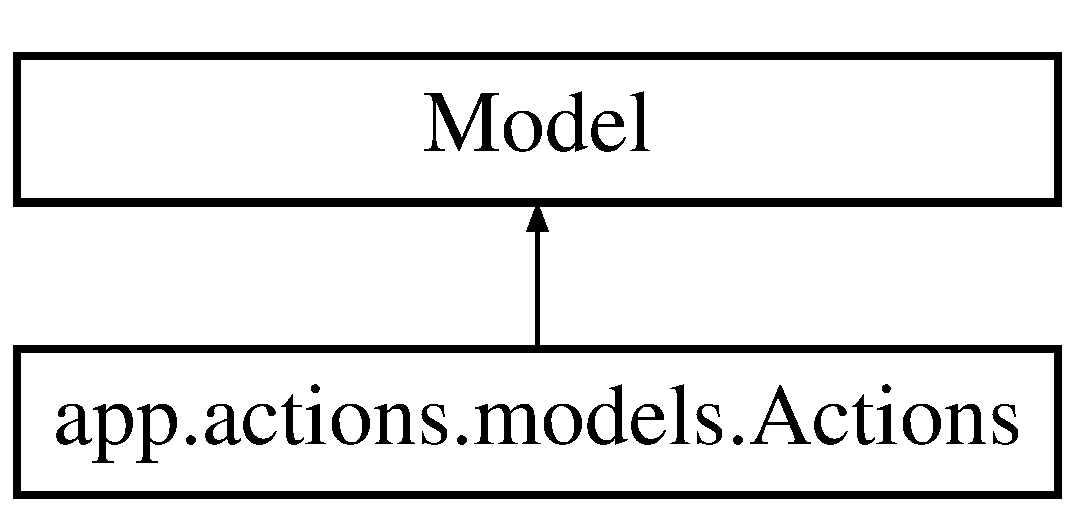
\includegraphics[height=2.000000cm]{classapp_1_1actions_1_1models_1_1_actions}
\end{center}
\end{figure}
\subsection*{Static Public Attributes}
\begin{DoxyCompactItemize}
\item 
\mbox{\Hypertarget{classapp_1_1actions_1_1models_1_1_actions_ad5102328491b54276b56c31d1f222f0c}\label{classapp_1_1actions_1_1models_1_1_actions_ad5102328491b54276b56c31d1f222f0c}} 
{\bfseries id} = db.\+Column(db.\+Integer, primary\+\_\+key=True, unique=True)
\item 
\mbox{\Hypertarget{classapp_1_1actions_1_1models_1_1_actions_ad48ceed71ad831eb40c92f862d829c79}\label{classapp_1_1actions_1_1models_1_1_actions_ad48ceed71ad831eb40c92f862d829c79}} 
{\bfseries title} = db.\+Column(db.\+String(255))
\item 
\mbox{\Hypertarget{classapp_1_1actions_1_1models_1_1_actions_a88fa96fe039a99483fa24bdcef4d3326}\label{classapp_1_1actions_1_1models_1_1_actions_a88fa96fe039a99483fa24bdcef4d3326}} 
{\bfseries description} = db.\+Column(db.\+String)
\item 
\mbox{\Hypertarget{classapp_1_1actions_1_1models_1_1_actions_a9a101aea1ba6da349bdfc95385c02f67}\label{classapp_1_1actions_1_1models_1_1_actions_a9a101aea1ba6da349bdfc95385c02f67}} 
{\bfseries assigned\+\_\+to} = db.\+Column(db.\+Foreign\+Key(\textquotesingle{}users.\+id\textquotesingle{}))
\item 
\mbox{\Hypertarget{classapp_1_1actions_1_1models_1_1_actions_a3e430c7d110773a03facd6e7284a6512}\label{classapp_1_1actions_1_1models_1_1_actions_a3e430c7d110773a03facd6e7284a6512}} 
{\bfseries charge} = db.\+Column(db.\+Foreign\+Key(\textquotesingle{}charges.\+id\textquotesingle{}))
\item 
\mbox{\Hypertarget{classapp_1_1actions_1_1models_1_1_actions_af92e45f68009abdced71b9bb2f71a71b}\label{classapp_1_1actions_1_1models_1_1_actions_af92e45f68009abdced71b9bb2f71a71b}} 
{\bfseries notes} = db.\+relationship(\textquotesingle{}\mbox{\hyperlink{classapp_1_1notes_1_1models_1_1_notes}{Notes}}\textquotesingle{}, backref=\textquotesingle{}actions\textquotesingle{}, lazy=\textquotesingle{}dynamic\textquotesingle{})
\item 
\mbox{\Hypertarget{classapp_1_1actions_1_1models_1_1_actions_a5d28004f4e6b3a38da8d522b3a984070}\label{classapp_1_1actions_1_1models_1_1_actions_a5d28004f4e6b3a38da8d522b3a984070}} 
{\bfseries created\+\_\+at} = db.\+Column(db.\+Date\+Time, server\+\_\+default= db.\+func.\+now())
\item 
list {\bfseries status\+\_\+types}
\item 
\mbox{\Hypertarget{classapp_1_1actions_1_1models_1_1_actions_aec5f6fed0f4febda1e7dd3ac45af5026}\label{classapp_1_1actions_1_1models_1_1_actions_aec5f6fed0f4febda1e7dd3ac45af5026}} 
{\bfseries action\+\_\+status} = db.\+Column(Choice\+Type(status\+\_\+types))
\end{DoxyCompactItemize}


\subsection{Member Data Documentation}
\mbox{\Hypertarget{classapp_1_1actions_1_1models_1_1_actions_aff60531385518f41d1aec340f0e2cf2f}\label{classapp_1_1actions_1_1models_1_1_actions_aff60531385518f41d1aec340f0e2cf2f}} 
\index{app\+::actions\+::models\+::\+Actions@{app\+::actions\+::models\+::\+Actions}!status\+\_\+types@{status\+\_\+types}}
\index{status\+\_\+types@{status\+\_\+types}!app\+::actions\+::models\+::\+Actions@{app\+::actions\+::models\+::\+Actions}}
\subsubsection{\texorpdfstring{status\+\_\+types}{status\_types}}
{\footnotesize\ttfamily list app.\+actions.\+models.\+Actions.\+status\+\_\+types\hspace{0.3cm}{\ttfamily [static]}}

{\bfseries Initial value\+:}
\begin{DoxyCode}
=  [(0, \textcolor{stringliteral}{"In Progress"}), (1, \textcolor{stringliteral}{"Indefinite"}), (2, \textcolor{stringliteral}{"Unknown"}),
                    (3, \textcolor{stringliteral}{"Completed"}), (4, \textcolor{stringliteral}{"Stopped"}), (5, \textcolor{stringliteral}{"Incomplete"}), (6, \textcolor{stringliteral}{"On Hold"})]
\end{DoxyCode}


The documentation for this class was generated from the following file\+:\begin{DoxyCompactItemize}
\item 
app/actions/models.\+py\end{DoxyCompactItemize}

\hypertarget{classapp_1_1charges_1_1models_1_1_charges}{}\section{app.\+charges.\+models.\+Charges Class Reference}
\label{classapp_1_1charges_1_1models_1_1_charges}\index{app.\+charges.\+models.\+Charges@{app.\+charges.\+models.\+Charges}}


\mbox{\hyperlink{classapp_1_1charges_1_1models_1_1_charges}{Charges}} Model.  


Inheritance diagram for app.\+charges.\+models.\+Charges\+:\begin{figure}[H]
\begin{center}
\leavevmode
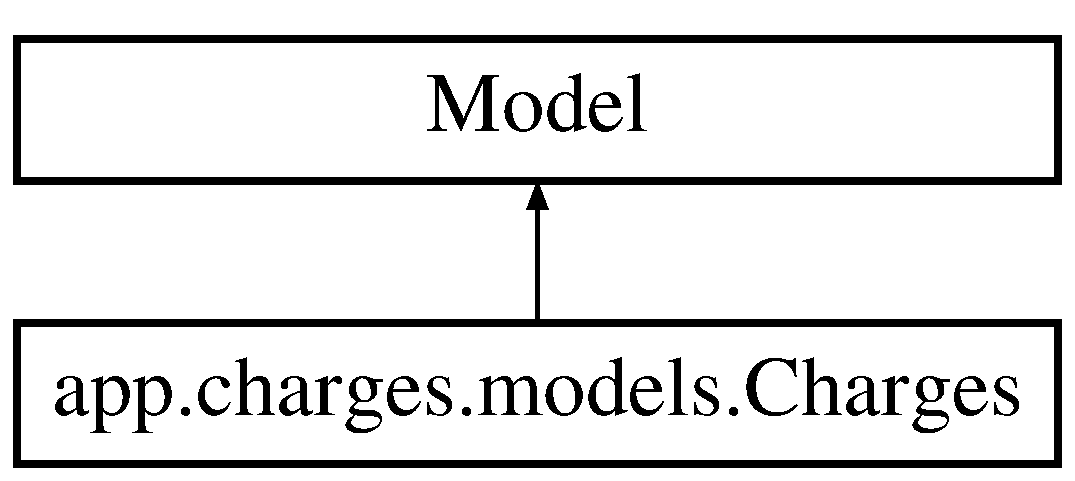
\includegraphics[height=2.000000cm]{classapp_1_1charges_1_1models_1_1_charges}
\end{center}
\end{figure}
\subsection*{Static Public Attributes}
\begin{DoxyCompactItemize}
\item 
\mbox{\Hypertarget{classapp_1_1charges_1_1models_1_1_charges_af54c5389801c1e7324e70d0a7db11f8f}\label{classapp_1_1charges_1_1models_1_1_charges_af54c5389801c1e7324e70d0a7db11f8f}} 
{\bfseries id} = db.\+Column(db.\+Integer, primary\+\_\+key=True, unique=True)
\item 
\mbox{\Hypertarget{classapp_1_1charges_1_1models_1_1_charges_ad8ff9ab21dbae0938197587fc91a3691}\label{classapp_1_1charges_1_1models_1_1_charges_ad8ff9ab21dbae0938197587fc91a3691}} 
{\bfseries title} = db.\+Column(db.\+String(255))
\item 
\mbox{\Hypertarget{classapp_1_1charges_1_1models_1_1_charges_a3d780746fc539306a6b7e0e0f356817e}\label{classapp_1_1charges_1_1models_1_1_charges_a3d780746fc539306a6b7e0e0f356817e}} 
{\bfseries author} = db.\+Column(db.\+Foreign\+Key(\textquotesingle{}users.\+id\textquotesingle{}))
\item 
\mbox{\Hypertarget{classapp_1_1charges_1_1models_1_1_charges_a696c6a3c010790e2d1337280957c6c39}\label{classapp_1_1charges_1_1models_1_1_charges_a696c6a3c010790e2d1337280957c6c39}} 
{\bfseries description} = db.\+Column(db.\+String(255))
\item 
\mbox{\Hypertarget{classapp_1_1charges_1_1models_1_1_charges_ab21d1af035df05a55e970114df4b8770}\label{classapp_1_1charges_1_1models_1_1_charges_ab21d1af035df05a55e970114df4b8770}} 
{\bfseries created\+\_\+at} = db.\+Column(db.\+Date\+Time, server\+\_\+default= db.\+func.\+now())
\item 
\mbox{\Hypertarget{classapp_1_1charges_1_1models_1_1_charges_adc62a6fe0f9cb978149336a372ac4b7a}\label{classapp_1_1charges_1_1models_1_1_charges_adc62a6fe0f9cb978149336a372ac4b7a}} 
{\bfseries committee} = db.\+Column(db.\+Foreign\+Key(\textquotesingle{}committees.\+id\textquotesingle{}))
\item 
\mbox{\Hypertarget{classapp_1_1charges_1_1models_1_1_charges_a45c59f4fe0b91b2cb598d24d0cfa72be}\label{classapp_1_1charges_1_1models_1_1_charges_a45c59f4fe0b91b2cb598d24d0cfa72be}} 
{\bfseries objectives} = db.\+Column(A\+R\+R\+AY(db.\+String))
\item 
\mbox{\Hypertarget{classapp_1_1charges_1_1models_1_1_charges_a51f84a59feeef986ef40e4e43d235aa6}\label{classapp_1_1charges_1_1models_1_1_charges_a51f84a59feeef986ef40e4e43d235aa6}} 
{\bfseries schedule} = db.\+Column(A\+R\+R\+AY(db.\+String))
\item 
\mbox{\Hypertarget{classapp_1_1charges_1_1models_1_1_charges_aa8690b0bc424efdd2c84baf90eace781}\label{classapp_1_1charges_1_1models_1_1_charges_aa8690b0bc424efdd2c84baf90eace781}} 
{\bfseries actions} = db.\+relationship(\textquotesingle{}\mbox{\hyperlink{classapp_1_1actions_1_1models_1_1_actions}{Actions}}\textquotesingle{}, backref=\textquotesingle{}charges\textquotesingle{}, lazy=\textquotesingle{}dynamic\textquotesingle{})
\item 
\mbox{\Hypertarget{classapp_1_1charges_1_1models_1_1_charges_a6ea2d6327d1d6cb5dc016ccede60a788}\label{classapp_1_1charges_1_1models_1_1_charges_a6ea2d6327d1d6cb5dc016ccede60a788}} 
{\bfseries resources} = db.\+Column(A\+R\+R\+AY(db.\+String))
\item 
\mbox{\Hypertarget{classapp_1_1charges_1_1models_1_1_charges_ac530dc2cb9ecf1edd5cb12e7aa3eb06e}\label{classapp_1_1charges_1_1models_1_1_charges_ac530dc2cb9ecf1edd5cb12e7aa3eb06e}} 
{\bfseries stakeholders} = db.\+Column(A\+R\+R\+AY(db.\+String))
\item 
\mbox{\Hypertarget{classapp_1_1charges_1_1models_1_1_charges_a8d32e2c6e5fb5995c2bce2e3ec9ceb69}\label{classapp_1_1charges_1_1models_1_1_charges_a8d32e2c6e5fb5995c2bce2e3ec9ceb69}} 
{\bfseries priority} = db.\+Column(Choice\+Type(\mbox{\hyperlink{classapp_1_1charges_1_1models_1_1_priority_type}{Priority\+Type}}))
\item 
\mbox{\Hypertarget{classapp_1_1charges_1_1models_1_1_charges_aacd52559619e5d6a20706e2ac269e41b}\label{classapp_1_1charges_1_1models_1_1_charges_aacd52559619e5d6a20706e2ac269e41b}} 
{\bfseries status} = db.\+Column(Choice\+Type(\mbox{\hyperlink{classapp_1_1charges_1_1models_1_1_status_type}{Status\+Type}}))
\end{DoxyCompactItemize}


\subsection{Detailed Description}
\mbox{\hyperlink{classapp_1_1charges_1_1models_1_1_charges}{Charges}} Model. 

The documentation for this class was generated from the following file\+:\begin{DoxyCompactItemize}
\item 
app/charges/models.\+py\end{DoxyCompactItemize}

\hypertarget{classapp_1_1committees_1_1models_1_1_committees}{}\section{app.\+committees.\+models.\+Committees Class Reference}
\label{classapp_1_1committees_1_1models_1_1_committees}\index{app.\+committees.\+models.\+Committees@{app.\+committees.\+models.\+Committees}}
Inheritance diagram for app.\+committees.\+models.\+Committees\+:\begin{figure}[H]
\begin{center}
\leavevmode
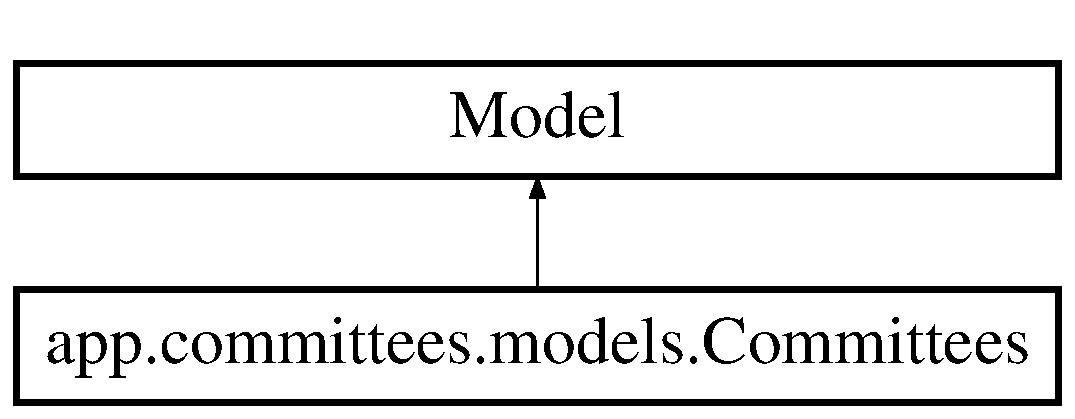
\includegraphics[height=2.000000cm]{classapp_1_1committees_1_1models_1_1_committees}
\end{center}
\end{figure}
\subsection*{Static Public Attributes}
\begin{DoxyCompactItemize}
\item 
\mbox{\Hypertarget{classapp_1_1committees_1_1models_1_1_committees_a3c8aed6bb6326fc3ac1331e650416d69}\label{classapp_1_1committees_1_1models_1_1_committees_a3c8aed6bb6326fc3ac1331e650416d69}} 
{\bfseries id} = db.\+Column(db.\+String(255), primary\+\_\+key=True, unique= True)
\item 
\mbox{\Hypertarget{classapp_1_1committees_1_1models_1_1_committees_a0f6412a1d895d1c00128c7a3cf858854}\label{classapp_1_1committees_1_1models_1_1_committees_a0f6412a1d895d1c00128c7a3cf858854}} 
{\bfseries title} = db.\+Column(db.\+String(255))
\item 
\mbox{\Hypertarget{classapp_1_1committees_1_1models_1_1_committees_a675ede01d1ee8ccf632ed50c3e02316e}\label{classapp_1_1committees_1_1models_1_1_committees_a675ede01d1ee8ccf632ed50c3e02316e}} 
{\bfseries description} = db.\+Column(db.\+String(255))
\item 
\mbox{\Hypertarget{classapp_1_1committees_1_1models_1_1_committees_aca3664e78077e6605292261f99d3a645}\label{classapp_1_1committees_1_1models_1_1_committees_aca3664e78077e6605292261f99d3a645}} 
{\bfseries head} = db.\+Column(db.\+Foreign\+Key(\textquotesingle{}users.\+id\textquotesingle{}))
\item 
\mbox{\Hypertarget{classapp_1_1committees_1_1models_1_1_committees_a84dc8b2bf2e7ea7eb56e6131d536f26e}\label{classapp_1_1committees_1_1models_1_1_committees_a84dc8b2bf2e7ea7eb56e6131d536f26e}} 
{\bfseries location} = db.\+Column(db.\+String(255))
\item 
\mbox{\Hypertarget{classapp_1_1committees_1_1models_1_1_committees_add56310ed392f463e3827ba5d67cd945}\label{classapp_1_1committees_1_1models_1_1_committees_add56310ed392f463e3827ba5d67cd945}} 
{\bfseries committee\+\_\+img} = db.\+Column(db.\+Large\+Binary)
\item 
\mbox{\Hypertarget{classapp_1_1committees_1_1models_1_1_committees_afe19cf4d32d65902f27b2ee42736bb2a}\label{classapp_1_1committees_1_1models_1_1_committees_afe19cf4d32d65902f27b2ee42736bb2a}} 
{\bfseries meeting\+\_\+time} = db.\+Column(db.\+String(4))
\item 
\mbox{\Hypertarget{classapp_1_1committees_1_1models_1_1_committees_a6c8539a3799bf491d821df4c8aa1ef8f}\label{classapp_1_1committees_1_1models_1_1_committees_a6c8539a3799bf491d821df4c8aa1ef8f}} 
{\bfseries meeting\+\_\+day} = db.\+Column(db.\+Integer)
\item 
\mbox{\Hypertarget{classapp_1_1committees_1_1models_1_1_committees_add464a66ef18f66a6129516fb6a507e3}\label{classapp_1_1committees_1_1models_1_1_committees_add464a66ef18f66a6129516fb6a507e3}} 
{\bfseries enabled} = db.\+Column(db.\+Boolean, default= True)
\end{DoxyCompactItemize}


The documentation for this class was generated from the following file\+:\begin{DoxyCompactItemize}
\item 
app/committees/models.\+py\end{DoxyCompactItemize}

\hypertarget{classapp_1_1invitations_1_1models_1_1_invitations}{}\section{app.\+invitations.\+models.\+Invitations Class Reference}
\label{classapp_1_1invitations_1_1models_1_1_invitations}\index{app.\+invitations.\+models.\+Invitations@{app.\+invitations.\+models.\+Invitations}}
Inheritance diagram for app.\+invitations.\+models.\+Invitations\+:\begin{figure}[H]
\begin{center}
\leavevmode
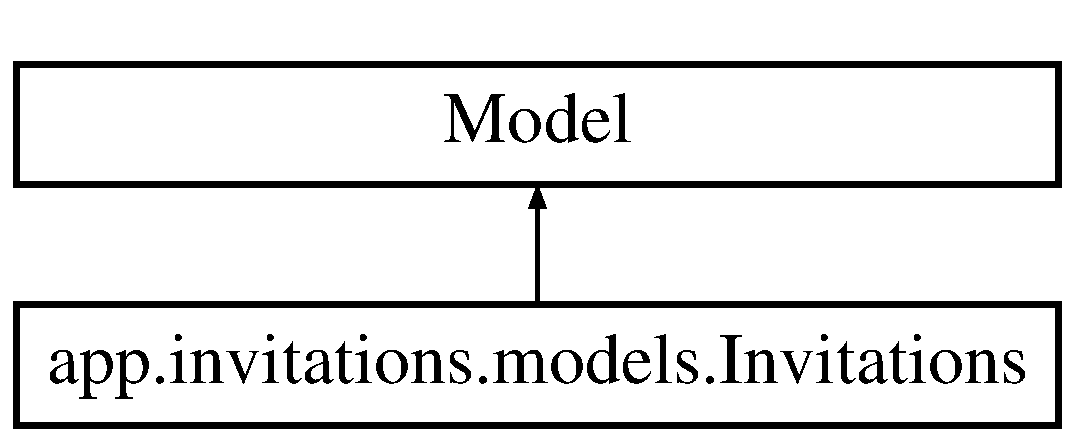
\includegraphics[height=2.000000cm]{classapp_1_1invitations_1_1models_1_1_invitations}
\end{center}
\end{figure}
\subsection*{Static Public Attributes}
\begin{DoxyCompactItemize}
\item 
\mbox{\Hypertarget{classapp_1_1invitations_1_1models_1_1_invitations_a0eb799f4087b5e18e7522b37a23066a1}\label{classapp_1_1invitations_1_1models_1_1_invitations_a0eb799f4087b5e18e7522b37a23066a1}} 
{\bfseries id} = db.\+Column(db.\+Integer, primary\+\_\+key=True, autoincrement=True)
\item 
\mbox{\Hypertarget{classapp_1_1invitations_1_1models_1_1_invitations_aaa400730c8069ee7cfc19e4cd7dd85fb}\label{classapp_1_1invitations_1_1models_1_1_invitations_aaa400730c8069ee7cfc19e4cd7dd85fb}} 
{\bfseries user\+\_\+name} = db.\+Column(db.\+String(255))
\item 
\mbox{\Hypertarget{classapp_1_1invitations_1_1models_1_1_invitations_a85959c0ec548e4fb861e8d760df34b80}\label{classapp_1_1invitations_1_1models_1_1_invitations_a85959c0ec548e4fb861e8d760df34b80}} 
{\bfseries committee\+\_\+id} = db.\+Column(db.\+Foreign\+Key(\textquotesingle{}committees.\+id\textquotesingle{}))
\item 
\mbox{\Hypertarget{classapp_1_1invitations_1_1models_1_1_invitations_ad1460453cca5b85ddf1fd094359919c0}\label{classapp_1_1invitations_1_1models_1_1_invitations_ad1460453cca5b85ddf1fd094359919c0}} 
{\bfseries committee} = db.\+relationship(\mbox{\hyperlink{classapp_1_1committees_1_1models_1_1_committees}{Committees}})
\item 
\mbox{\Hypertarget{classapp_1_1invitations_1_1models_1_1_invitations_a0458a9aa33004e79c5043090009da9f5}\label{classapp_1_1invitations_1_1models_1_1_invitations_a0458a9aa33004e79c5043090009da9f5}} 
{\bfseries is\+Invite} = db.\+Column(db.\+Boolean)
\end{DoxyCompactItemize}


The documentation for this class was generated from the following file\+:\begin{DoxyCompactItemize}
\item 
app/invitations/models.\+py\end{DoxyCompactItemize}

\hypertarget{classapp_1_1notes_1_1models_1_1_notes}{}\section{app.\+notes.\+models.\+Notes Class Reference}
\label{classapp_1_1notes_1_1models_1_1_notes}\index{app.\+notes.\+models.\+Notes@{app.\+notes.\+models.\+Notes}}
Inheritance diagram for app.\+notes.\+models.\+Notes\+:\begin{figure}[H]
\begin{center}
\leavevmode
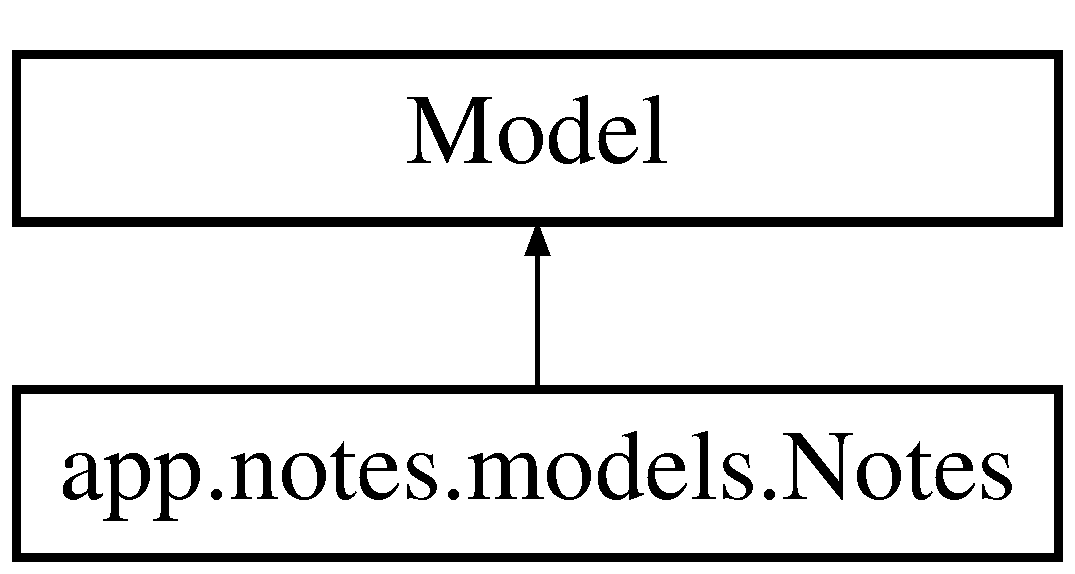
\includegraphics[height=2.000000cm]{classapp_1_1notes_1_1models_1_1_notes}
\end{center}
\end{figure}
\subsection*{Static Public Attributes}
\begin{DoxyCompactItemize}
\item 
\mbox{\Hypertarget{classapp_1_1notes_1_1models_1_1_notes_a0fab9aac35077f9e24ebb1558b0da526}\label{classapp_1_1notes_1_1models_1_1_notes_a0fab9aac35077f9e24ebb1558b0da526}} 
{\bfseries id} = db.\+Column(db.\+Integer, primary\+\_\+key=True, unique=True)
\item 
\mbox{\Hypertarget{classapp_1_1notes_1_1models_1_1_notes_a5b5ee3dc95f1e974c9aa5acce203857a}\label{classapp_1_1notes_1_1models_1_1_notes_a5b5ee3dc95f1e974c9aa5acce203857a}} 
{\bfseries description} = db.\+Column(db.\+String)
\item 
\mbox{\Hypertarget{classapp_1_1notes_1_1models_1_1_notes_a4dc95eb68a8fd9abc1f04f7546b23a93}\label{classapp_1_1notes_1_1models_1_1_notes_a4dc95eb68a8fd9abc1f04f7546b23a93}} 
{\bfseries author} = db.\+Column(db.\+Foreign\+Key(\textquotesingle{}users.\+id\textquotesingle{}))
\item 
\mbox{\Hypertarget{classapp_1_1notes_1_1models_1_1_notes_aae6677abfdc262d93bf1ef05788499cd}\label{classapp_1_1notes_1_1models_1_1_notes_aae6677abfdc262d93bf1ef05788499cd}} 
{\bfseries action} = db.\+Column(db.\+Foreign\+Key(\textquotesingle{}actions.\+id\textquotesingle{}))
\item 
\mbox{\Hypertarget{classapp_1_1notes_1_1models_1_1_notes_a2df3204b65153089aecdfc9710f35f1c}\label{classapp_1_1notes_1_1models_1_1_notes_a2df3204b65153089aecdfc9710f35f1c}} 
{\bfseries created\+\_\+at} = db.\+Column(db.\+Date\+Time, server\+\_\+default= db.\+func.\+now())
\end{DoxyCompactItemize}


The documentation for this class was generated from the following file\+:\begin{DoxyCompactItemize}
\item 
app/notes/models.\+py\end{DoxyCompactItemize}

\hypertarget{classapp_1_1users_1_1permissions_1_1_permissions}{}\section{app.\+users.\+permissions.\+Permissions Class Reference}
\label{classapp_1_1users_1_1permissions_1_1_permissions}\index{app.\+users.\+permissions.\+Permissions@{app.\+users.\+permissions.\+Permissions}}


Permission categories for users.  


\subsection*{Static Public Attributes}
\begin{DoxyCompactItemize}
\item 
int \mbox{\hyperlink{classapp_1_1users_1_1permissions_1_1_permissions_a91cbb1b3d525ea47ffe4b5b12bfe979e}{Can\+Edit}} = 4
\begin{DoxyCompactList}\small\item\em Change heads, status, remove members and transfer charges. \end{DoxyCompactList}\item 
int \mbox{\hyperlink{classapp_1_1users_1_1permissions_1_1_permissions_aabbe27ce336c3209218a350fd4a46425}{Can\+Create}} = 3
\begin{DoxyCompactList}\small\item\em Can create Actions. \end{DoxyCompactList}\item 
int \mbox{\hyperlink{classapp_1_1users_1_1permissions_1_1_permissions_a473f3e4b52e00caaac924ebe2967f398}{Can\+Contribute}} = 2
\begin{DoxyCompactList}\small\item\em View actions, create notes and charges. \end{DoxyCompactList}\item 
int \mbox{\hyperlink{classapp_1_1users_1_1permissions_1_1_permissions_af5c7edc65060e65ac211996e10c5809a}{Can\+View}} = 1
\begin{DoxyCompactList}\small\item\em View changes in Committees. \end{DoxyCompactList}\end{DoxyCompactItemize}


\subsection{Detailed Description}
Permission categories for users. 

A bigger permission number contains the privileges of a lesser number.


\begin{DoxyItemize}
\item Can\+View\+: View changes in Committees.
\item Can\+Contribute\+: View actions, create notes and charges.
\item Can\+Create\+: Can create Actions.
\item Can\+Edit\+: Can change heads, change status, remove members and transfer charges. 
\end{DoxyItemize}

\subsection{Member Data Documentation}
\mbox{\Hypertarget{classapp_1_1users_1_1permissions_1_1_permissions_a473f3e4b52e00caaac924ebe2967f398}\label{classapp_1_1users_1_1permissions_1_1_permissions_a473f3e4b52e00caaac924ebe2967f398}} 
\index{app\+::users\+::permissions\+::\+Permissions@{app\+::users\+::permissions\+::\+Permissions}!Can\+Contribute@{Can\+Contribute}}
\index{Can\+Contribute@{Can\+Contribute}!app\+::users\+::permissions\+::\+Permissions@{app\+::users\+::permissions\+::\+Permissions}}
\subsubsection{\texorpdfstring{Can\+Contribute}{CanContribute}}
{\footnotesize\ttfamily int app.\+users.\+permissions.\+Permissions.\+Can\+Contribute = 2\hspace{0.3cm}{\ttfamily [static]}}



View actions, create notes and charges. 

\mbox{\Hypertarget{classapp_1_1users_1_1permissions_1_1_permissions_aabbe27ce336c3209218a350fd4a46425}\label{classapp_1_1users_1_1permissions_1_1_permissions_aabbe27ce336c3209218a350fd4a46425}} 
\index{app\+::users\+::permissions\+::\+Permissions@{app\+::users\+::permissions\+::\+Permissions}!Can\+Create@{Can\+Create}}
\index{Can\+Create@{Can\+Create}!app\+::users\+::permissions\+::\+Permissions@{app\+::users\+::permissions\+::\+Permissions}}
\subsubsection{\texorpdfstring{Can\+Create}{CanCreate}}
{\footnotesize\ttfamily int app.\+users.\+permissions.\+Permissions.\+Can\+Create = 3\hspace{0.3cm}{\ttfamily [static]}}



Can create Actions. 

\mbox{\Hypertarget{classapp_1_1users_1_1permissions_1_1_permissions_a91cbb1b3d525ea47ffe4b5b12bfe979e}\label{classapp_1_1users_1_1permissions_1_1_permissions_a91cbb1b3d525ea47ffe4b5b12bfe979e}} 
\index{app\+::users\+::permissions\+::\+Permissions@{app\+::users\+::permissions\+::\+Permissions}!Can\+Edit@{Can\+Edit}}
\index{Can\+Edit@{Can\+Edit}!app\+::users\+::permissions\+::\+Permissions@{app\+::users\+::permissions\+::\+Permissions}}
\subsubsection{\texorpdfstring{Can\+Edit}{CanEdit}}
{\footnotesize\ttfamily int app.\+users.\+permissions.\+Permissions.\+Can\+Edit = 4\hspace{0.3cm}{\ttfamily [static]}}



Change heads, status, remove members and transfer charges. 

\mbox{\Hypertarget{classapp_1_1users_1_1permissions_1_1_permissions_af5c7edc65060e65ac211996e10c5809a}\label{classapp_1_1users_1_1permissions_1_1_permissions_af5c7edc65060e65ac211996e10c5809a}} 
\index{app\+::users\+::permissions\+::\+Permissions@{app\+::users\+::permissions\+::\+Permissions}!Can\+View@{Can\+View}}
\index{Can\+View@{Can\+View}!app\+::users\+::permissions\+::\+Permissions@{app\+::users\+::permissions\+::\+Permissions}}
\subsubsection{\texorpdfstring{Can\+View}{CanView}}
{\footnotesize\ttfamily int app.\+users.\+permissions.\+Permissions.\+Can\+View = 1\hspace{0.3cm}{\ttfamily [static]}}



View changes in Committees. 



The documentation for this class was generated from the following file\+:\begin{DoxyCompactItemize}
\item 
app/users/permissions.\+py\end{DoxyCompactItemize}

\hypertarget{classapp_1_1charges_1_1models_1_1_priority_type}{}\section{app.\+charges.\+models.\+Priority\+Type Class Reference}
\label{classapp_1_1charges_1_1models_1_1_priority_type}\index{app.\+charges.\+models.\+Priority\+Type@{app.\+charges.\+models.\+Priority\+Type}}


Levels of priority for charges.  


Inheritance diagram for app.\+charges.\+models.\+Priority\+Type\+:\begin{figure}[H]
\begin{center}
\leavevmode
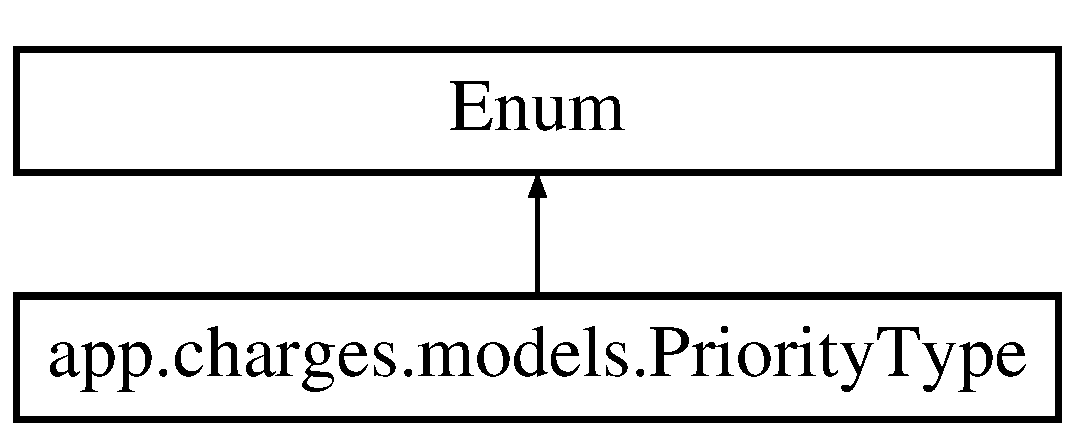
\includegraphics[height=2.000000cm]{classapp_1_1charges_1_1models_1_1_priority_type}
\end{center}
\end{figure}
\subsection*{Static Public Attributes}
\begin{DoxyCompactItemize}
\item 
\mbox{\Hypertarget{classapp_1_1charges_1_1models_1_1_priority_type_a677336d553eb0c071bf3545aba8653a8}\label{classapp_1_1charges_1_1models_1_1_priority_type_a677336d553eb0c071bf3545aba8653a8}} 
int {\bfseries Low} = 0
\item 
\mbox{\Hypertarget{classapp_1_1charges_1_1models_1_1_priority_type_aa9276e7802525f37029da2ea258ca611}\label{classapp_1_1charges_1_1models_1_1_priority_type_aa9276e7802525f37029da2ea258ca611}} 
int {\bfseries Medium} = 1
\item 
\mbox{\Hypertarget{classapp_1_1charges_1_1models_1_1_priority_type_a024f234040f34676358bacbcf35981a7}\label{classapp_1_1charges_1_1models_1_1_priority_type_a024f234040f34676358bacbcf35981a7}} 
int {\bfseries High} = 2
\end{DoxyCompactItemize}


\subsection{Detailed Description}
Levels of priority for charges. 

The documentation for this class was generated from the following file\+:\begin{DoxyCompactItemize}
\item 
app/charges/models.\+py\end{DoxyCompactItemize}

\hypertarget{classapp_1_1charges_1_1models_1_1_status_type}{}\section{app.\+charges.\+models.\+Status\+Type Class Reference}
\label{classapp_1_1charges_1_1models_1_1_status_type}\index{app.\+charges.\+models.\+Status\+Type@{app.\+charges.\+models.\+Status\+Type}}


Status types for charges.  


Inheritance diagram for app.\+charges.\+models.\+Status\+Type\+:\begin{figure}[H]
\begin{center}
\leavevmode
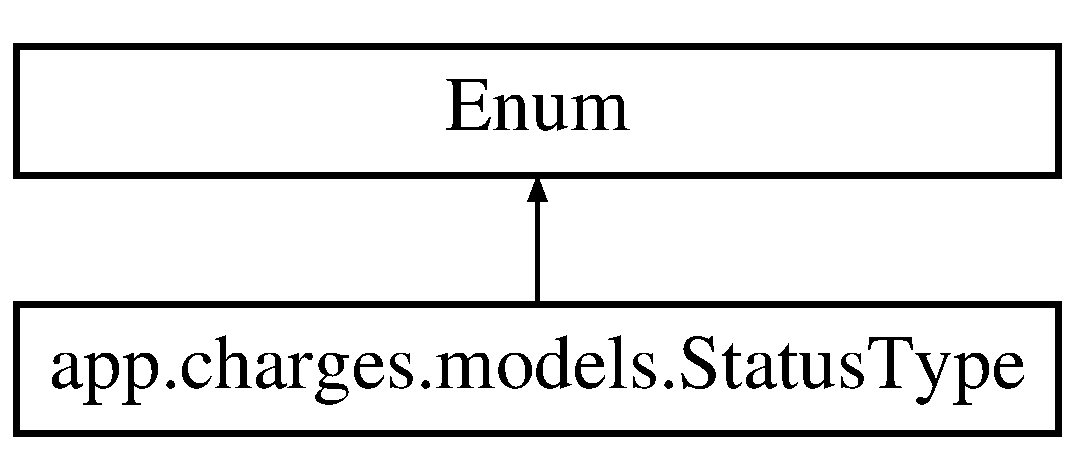
\includegraphics[height=2.000000cm]{classapp_1_1charges_1_1models_1_1_status_type}
\end{center}
\end{figure}
\subsection*{Static Public Attributes}
\begin{DoxyCompactItemize}
\item 
\mbox{\Hypertarget{classapp_1_1charges_1_1models_1_1_status_type_a2bf05f149fd78d609ca9baba78886c68}\label{classapp_1_1charges_1_1models_1_1_status_type_a2bf05f149fd78d609ca9baba78886c68}} 
int {\bfseries Unapproved} = 0
\item 
\mbox{\Hypertarget{classapp_1_1charges_1_1models_1_1_status_type_a60b90f5febb9da5281f6d2a2f9f6d671}\label{classapp_1_1charges_1_1models_1_1_status_type_a60b90f5febb9da5281f6d2a2f9f6d671}} 
int {\bfseries Failed} = 1
\item 
\mbox{\Hypertarget{classapp_1_1charges_1_1models_1_1_status_type_abc57b85f75f07de1021f80b0507ffb87}\label{classapp_1_1charges_1_1models_1_1_status_type_abc57b85f75f07de1021f80b0507ffb87}} 
int {\bfseries In\+Progress} = 2
\item 
\mbox{\Hypertarget{classapp_1_1charges_1_1models_1_1_status_type_a1274e714ca7dca6fd6e5c7cb5dcc751c}\label{classapp_1_1charges_1_1models_1_1_status_type_a1274e714ca7dca6fd6e5c7cb5dcc751c}} 
int {\bfseries Indefinite} = 3
\item 
\mbox{\Hypertarget{classapp_1_1charges_1_1models_1_1_status_type_abaf74561902ff9d02600769c5176c560}\label{classapp_1_1charges_1_1models_1_1_status_type_abaf74561902ff9d02600769c5176c560}} 
int {\bfseries Unknown} = 4
\item 
\mbox{\Hypertarget{classapp_1_1charges_1_1models_1_1_status_type_af5c57965eb7cf4589e19e6f1cdf43d64}\label{classapp_1_1charges_1_1models_1_1_status_type_af5c57965eb7cf4589e19e6f1cdf43d64}} 
int {\bfseries Completed} = 5
\item 
\mbox{\Hypertarget{classapp_1_1charges_1_1models_1_1_status_type_a1198d8722f0daa3f82f6ff69d88b0275}\label{classapp_1_1charges_1_1models_1_1_status_type_a1198d8722f0daa3f82f6ff69d88b0275}} 
int {\bfseries Not\+Started} = 6
\item 
\mbox{\Hypertarget{classapp_1_1charges_1_1models_1_1_status_type_a7c7b79a3607c74522411acff4525f146}\label{classapp_1_1charges_1_1models_1_1_status_type_a7c7b79a3607c74522411acff4525f146}} 
int {\bfseries Stopped} = 7
\end{DoxyCompactItemize}


\subsection{Detailed Description}
Status types for charges. 

The documentation for this class was generated from the following file\+:\begin{DoxyCompactItemize}
\item 
app/charges/models.\+py\end{DoxyCompactItemize}

\hypertarget{classapp_1_1users_1_1models_1_1_users}{}\section{app.\+users.\+models.\+Users Class Reference}
\label{classapp_1_1users_1_1models_1_1_users}\index{app.\+users.\+models.\+Users@{app.\+users.\+models.\+Users}}
Inheritance diagram for app.\+users.\+models.\+Users\+:\begin{figure}[H]
\begin{center}
\leavevmode
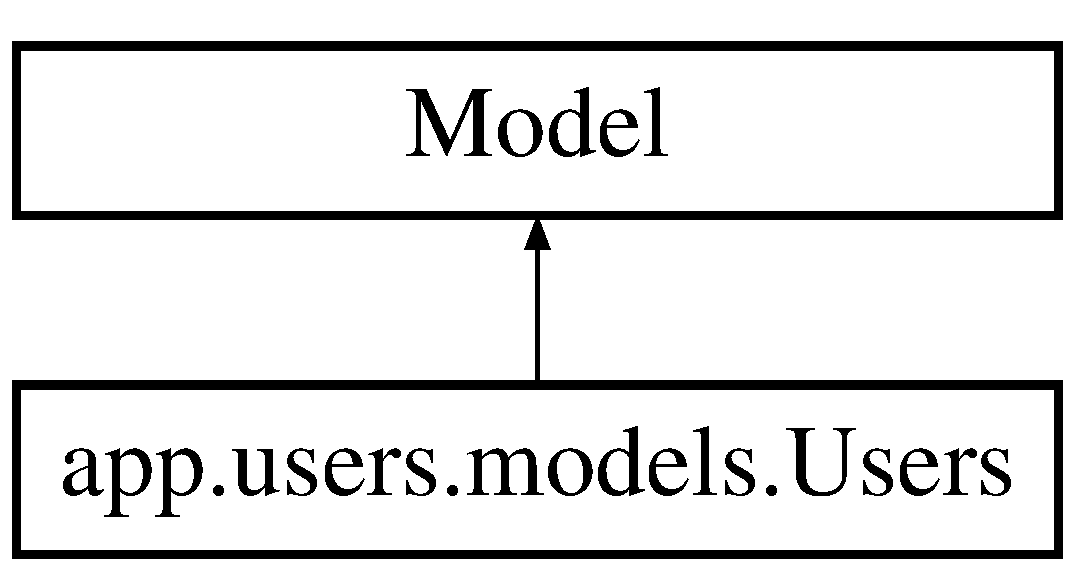
\includegraphics[height=2.000000cm]{classapp_1_1users_1_1models_1_1_users}
\end{center}
\end{figure}
\subsection*{Public Member Functions}
\begin{DoxyCompactItemize}
\item 
\mbox{\Hypertarget{classapp_1_1users_1_1models_1_1_users_a461b688805d8e521361ef1faf181b1ae}\label{classapp_1_1users_1_1models_1_1_users_a461b688805d8e521361ef1faf181b1ae}} 
def {\bfseries generate\+\_\+auth} (self, expiration=60000000000000)
\end{DoxyCompactItemize}
\subsection*{Static Public Member Functions}
\begin{DoxyCompactItemize}
\item 
\mbox{\Hypertarget{classapp_1_1users_1_1models_1_1_users_a1f04be66797fe5e857214ea0f4ab465d}\label{classapp_1_1users_1_1models_1_1_users_a1f04be66797fe5e857214ea0f4ab465d}} 
def {\bfseries verify\+\_\+auth} (token)
\end{DoxyCompactItemize}
\subsection*{Static Public Attributes}
\begin{DoxyCompactItemize}
\item 
\mbox{\Hypertarget{classapp_1_1users_1_1models_1_1_users_aa414198ce22897dcc0cb164e1e630f2e}\label{classapp_1_1users_1_1models_1_1_users_aa414198ce22897dcc0cb164e1e630f2e}} 
{\bfseries id} = db.\+Column(db.\+String, primary\+\_\+key=True, unique= True)
\item 
\mbox{\Hypertarget{classapp_1_1users_1_1models_1_1_users_a8a38223ace2166e20b7a1bbbd5d2fc16}\label{classapp_1_1users_1_1models_1_1_users_a8a38223ace2166e20b7a1bbbd5d2fc16}} 
{\bfseries first\+\_\+name} = db.\+Column(db.\+String(255))
\item 
\mbox{\Hypertarget{classapp_1_1users_1_1models_1_1_users_ab8b402194d4ae9decb5e5a1f7afb7c86}\label{classapp_1_1users_1_1models_1_1_users_ab8b402194d4ae9decb5e5a1f7afb7c86}} 
{\bfseries last\+\_\+name} = db.\+Column(db.\+String(255))
\item 
\mbox{\Hypertarget{classapp_1_1users_1_1models_1_1_users_a44d0472206bce2b5904fa1263f4c0349}\label{classapp_1_1users_1_1models_1_1_users_a44d0472206bce2b5904fa1263f4c0349}} 
{\bfseries email} = db.\+Column(db.\+String(255))
\item 
\mbox{\Hypertarget{classapp_1_1users_1_1models_1_1_users_aea04a132efcb104036de3ed2e33172fc}\label{classapp_1_1users_1_1models_1_1_users_aea04a132efcb104036de3ed2e33172fc}} 
{\bfseries is\+\_\+admin} = db.\+Column(db.\+Boolean)
\item 
\mbox{\Hypertarget{classapp_1_1users_1_1models_1_1_users_a1fbbe2145bdfa8ec81cdf8ebc270514b}\label{classapp_1_1users_1_1models_1_1_users_a1fbbe2145bdfa8ec81cdf8ebc270514b}} 
{\bfseries committees} = db.\+relationship(\textquotesingle{}\mbox{\hyperlink{classapp_1_1committees_1_1models_1_1_committees}{Committees}}\textquotesingle{}, secondary= members\+\_\+table, back\+\_\+populates= \textquotesingle{}members\textquotesingle{})
\end{DoxyCompactItemize}


The documentation for this class was generated from the following file\+:\begin{DoxyCompactItemize}
\item 
app/users/models.\+py\end{DoxyCompactItemize}

%--- End generated contents ---

% Index
\backmatter
\newpage
\phantomsection
\clearemptydoublepage
\addcontentsline{toc}{chapter}{Index}
\printindex

\end{document}
